\documentclass[11pt,a4paper]{article}

% Paquets de base
\usepackage[utf8]{inputenc}
\usepackage[T1]{fontenc}
\usepackage{lmodern}
\usepackage{microtype}
\usepackage[a4paper,margin=2.2cm]{geometry}
\usepackage{amsmath,amssymb,mathtools}
\usepackage{graphicx}
\graphicspath{{../}} % les figures sont dans reports/figures
\usepackage{booktabs}
\usepackage{array}
\usepackage{tabularx}
\usepackage{multirow}
\usepackage{makecell}
\usepackage{enumitem}
\usepackage{xcolor}
\usepackage{float}
\usepackage{caption}
\usepackage{subcaption}

% Pseudocode
\usepackage{algorithm}
\usepackage{algpseudocode}
\algrenewcommand\algorithmicrequire{\textbf{Input:}}
\algrenewcommand\algorithmicensure{\textbf{Output:}}

% Références et Liens
\usepackage[hyphens]{url}
\usepackage{hyperref}
\usepackage[nameinlink,capitalise]{cleveref}

\hypersetup{
  colorlinks=true,
  linkcolor=blue!55!black,
  citecolor=blue!55!black,
  urlcolor=blue!65!black,
  pdftitle={Beyond Static Dispatching Heuristics},
  pdfauthor={Jean-Luc MUPASA KALUNGA}
}

% Configuration des légendes et tableaux
\captionsetup{font=small,labelfont=bf} % Légendes petites et labels en gras
\setlist[itemize]{leftmargin=1.5em,itemsep=2pt,topsep=4pt}
\setlist[enumerate]{leftmargin=1.7em,itemsep=2pt,topsep=4pt}
\renewcommand{\arraystretch}{1.15} % Espacement vertical des tableaux

% Suppression du style fancyhdr
\pagestyle{plain} 

% Macros de rédaction (optionnelles, mais gardées pour votre travail)
\newcommand{\pending}[1]{\textcolor{red}{[TO BE COMPLETED: #1]}}
\newcommand{\tbd}{\textcolor{red}{\textit{TBD}}}
% Cadre de figure provisoire (a remplacer par \includegraphics)
\newcommand{\phfig}[2][6cm]{%
  \fbox{\parbox[c][#1][c]{0.92\textwidth}{\centering\textit{#2}}}}

% Titre et Auteurs
\title{\textbf{Beyond Static Dispatching Heuristics: A Comparative Evaluation of Deep Reinforcement Learning under Disruptions in Open-Pit Mining}}

\author{%
\begin{tabular}{c}
Jean-Luc Mupasa Kalunga$^{1}$ \qquad Olfa Ferchichi$^{2}$\\[0.5em]
{\small $^{1}$Faculty of Computer Science, Don Bosco University of Lubumbashi (UDBL), Lubumbashi, DRC}\\
{\small $^{2}$RIADI Laboratory, ENSI, University of Manouba, Tunis, Tunisia}\\[0.3em]
{\small\texttt{16mk293@esisalama.org; olfaferchichi@yahoo.fr}}
\end{tabular}%
}
\date{} % Pas de date apparente


\begin{document}

\maketitle

\begin{abstract}
Truck--shovel systems account for up to 60\% of total operating costs in open-pit mining and are critically
sensitive to operational disruptions. Static dispatching heuristics remain the industry norm, and existing
reinforcement learning research typically evaluates policies under single-regime conditions, leaving the
resilience of adaptive agents under disruption poorly characterised.  This paper evaluates the performance and
operational robustness of eight dispatching policies: four classical heuristics, two tabular reinforcement
learning agents (Q-Learning, SARSA), and two deep reinforcement learning agents (Deep Q-Network (DQN),
Proximal Policy Optimization (PPO)), across three scenarios: nominal conditions, fleet oversaturation and high
equipment-failure frequency. Four primary performance indicators are assessed (productivity, average waiting time,
equipment utilisation and specific fuel consumption) using 30 independent replications per (policy, scenario)
pair and corrected statistical tests (Welch Analysis of Variance / Kruskal--Wallis, Holm--Bonferroni correction).  Three principal
findings emerge. First, PPO achieves the highest nominal productivity (4,176.7~t/h, $+2.6\%$ over Fixed Assignment,
$p < 0.001$, $d=1.94$). Second, a congestion collapse specific to distance-based heuristics is identified under
fleet oversaturation: Nearest Shovel and Shortest Path reach waiting times near 200 minutes per cycle, while
queue-based and deep reinforcement learning agents remain below 100 minutes.  Third, DQN delivers the highest
observed throughput under high-breakdown conditions (3,949.2~t/h), leading Fixed Assignment by 130.7~t/h (Dunn $p=5.78\times10^{-3}$, $d=1.896$); its 49.6~t/h advantage over PPO is not significant under the rank-based post-hoc test ($p=0.686$).  These results demonstrate that the benefits of deep reinforcement learning for truck
dispatching are strongly regime-dependent rather than universally superior to those of conventional heuristics.
PPO provides the highest productivity under nominal conditions, whereas Fixed Assignment remains highly competitive
under fleet oversaturation, and DQN exhibits the strongest absolute throughput under frequent equipment failures.
The observed reversal in policy rankings across operating regimes highlights the limitations of single-scenario
evaluation and supports the use of multi-regime stress-testing when assessing the operational resilience of
intelligent fleet-management policies.
\end{abstract}

\noindent\textbf{Keywords:} Deep reinforcement learning; Open-pit mining; Truck dispatching; Fleet management; Operational resilience; Stochastic simulation; PPO; DQN.

% ============================================================================
% Section 1: Introduction
% ============================================================================
\section{Introduction}
\label{sec:intro}

Open-pit mining represents a cornerstone of the global raw material supply chain, where the economic viability of operations is inextricably linked to the efficiency of large-scale logistical systems. Consequently, there is an imperative to explore recent technological advancements to enhance the performance and resilience of these logistical frameworks.

% ---------------------------------------------------------
\subsection{Industrial context}
% ---------------------------------------------------------

Open-pit mines are very large-scale industrial systems in which the truck--shovel cycle constitutes the main logistical backbone. This process, which involves the excavation, haulage and dumping of material, is not merely an operational task but a decisive financial driver, accounting for up to 60\% of the total operating costs of a mine site \cite{Afrapoli2017}. In modern mining, the pressure to optimise these flows is twofold: maximising throughput in order to meet global demand for raw materials, while minimising the energy consumption and greenhouse gas emissions associated with diesel haulage fleets.

The efficiency of these systems is, however, constantly challenged by strong operational variability. In real mining environments, conditions are far from deterministic. Equipment breakdowns, payload fluctuations, random travel times caused by road degradation and sudden traffic congestion together create a highly unstable environment. Managing this complexity requires real-time decision making capable of balancing immediate productivity against the long-term resilience of the fleet.

This study relies on three concepts that are used throughout the paper. \textit{Reinforcement Learning} (RL) designates a branch of artificial intelligence in which an autonomous agent learns optimal behaviour through trial-and-error interactions with a dynamic environment, so as to maximise a cumulative reward signal. \textit{Deep Reinforcement Learning} (DRL) extends RL by integrating deep neural networks to approximate value functions or policies, which allows the agent to handle the high-dimensional and continuous state spaces typical of mining infrastructures. \textit{Truck dispatching} designates the real-time operational process of assigning haulage units to specific loading and dumping locations in order to optimise fleet synchronisation and productivity.

% ---------------------------------------------------------
\subsection{Research problem}
\label{sec:problem-statement}
% ---------------------------------------------------------

The core dispatching challenge is the dynamic, real-time assignment of trucks to loading and dumping points so as to optimise a multi-dimensional objective that combines throughput, idle time and energy consumption. Fleet management systems (FMS) have been deployed in operating mines for several decades \cite{Afrapoli2017, AlexandraNewman2010}, and the decision rules that underpin them are well documented \cite{MohanMunirathinam1994, Alarie2002}.

These systems nevertheless struggle with the non-linearities induced by sudden disruptions. When a shovel breaks down or a haul road becomes congested, a local perturbation propagates across the entire haulage network, producing queue bottlenecks, under-utilisation of capital-intensive equipment and excessive fuel consumption during idling. Discrete-event studies of fleet oversaturation report this propagation effect and show that queueing time grows with fleet size once the loading capacity of the pit is exceeded \cite{Zeng2022, NecmettinCetin2004}.

The practical question that follows is not whether adaptive dispatching can improve productivity under stable conditions, but whether an adaptive policy remains preferable when the operating regime departs from the conditions under which it was designed. Answering that question requires comparing adaptive and rule-based policies under contrasting regimes, within one environment and one measurement protocol.

% ---------------------------------------------------------
\subsection{Research gap}
\label{sec:gap}
% ---------------------------------------------------------

The propagation effect described above has not been characterised across several disruption types under identical experimental conditions. Reviews of RL-based fleet management observe that most contributions remain at the proof-of-concept stage and are evaluated in stable environments \cite{Hazrathosseini2024}, and the individual studies confirm this pattern: agents are trained and tested under nominal conditions, against a small number of reference rules, and on a replication budget that is rarely reported \cite{deCarvalho2023, Zhao2025, Pei2025, FranciscoRosales2025}. The consequence is that a practitioner has no evidence base indicating under which operating conditions a learned dispatching policy should be deployed, and under which conditions a static heuristic remains the rational choice. \cref{sec:relwork} examines this gap in detail and \cref{sec:positioning} states how the present study addresses it.

% ---------------------------------------------------------
\subsection{Research questions and hypotheses}
\label{sec:rq}
% ---------------------------------------------------------

The empirical evaluation addresses the following research questions:

\begin{description}[leftmargin=1.2cm,labelwidth=1.0cm]

  \item[RQ1] Which dispatching policy achieves the highest productivity in each
  operational scenario, and does the ranking hold across scenarios?

  \item[RQ2] How does the trade-off between productivity and waiting time evolve
  from nominal to disrupted operating conditions?

  \item[RQ3] Are the observed performance gaps statistically significant after
  correction for multiple comparisons?

  \item[RQ4] How much do learned policies degrade when deployed on operating
  regimes that differ from the one used during training?

  \item[RQ5] How stable is the performance of each policy across independent
  random seeds?

  \item[RQ6] How does the choice of dispatching policy affect specific fuel
  consumption per tonne hauled, and does the ranking on this dimension follow
  the productivity ranking?

\end{description}

RQ1 is answered in \cref{sec:results}, RQ2 in \cref{sec:waiting}, RQ3 and RQ4 in \cref{sec:robustness} and the statistical analysis that follows it, RQ5 in \cref{sec:stability} and RQ6 in \cref{sec:sustainability}.

To guide this investigation, we formulate four falsifiable hypotheses:

\begin{itemize}
  \item \textbf{H1:} Deep reinforcement learning policies deliver higher productivity than static industrial heuristics under nominal operating conditions.
  \item \textbf{H2:} Under operational disruptions, deep reinforcement learning policies exhibit lower waiting-time degradation than static heuristics; their advantage on raw tonnage throughput is regime-dependent and is not guaranteed across all scenarios.
  \item \textbf{H3:} The optimal dispatching policy is regime-dependent; no single algorithm dominates in every operational state (nominal, high-load and high-breakdown).
  \item \textbf{H4:} High productivity is not necessarily correlated with low congestion, which suggests the existence of a Pareto trade-off between throughput and waiting times.
\end{itemize}

% ---------------------------------------------------------
\subsection{Contributions}
\label{sec:contributions}
% ---------------------------------------------------------

This work makes four contributions to mining engineering and intelligent fleet management. They are defended against the existing literature in \cref{sec:positioning} and instrumented in \cref{sec:design} and \cref{sec:results}.

\begin{itemize}
  \item \textbf{C1. Reproducible multi-regime evaluation framework.} A Gymnasium-compatible stochastic simulator is coupled with a standardised measurement protocol comprising 30 independent replications per (policy, scenario) pair, common random seeds for variance reduction, corrected omnibus and post-hoc tests, and bootstrap confidence intervals. To our knowledge, this is among the first openly available benchmarks for truck--shovel dispatching that cover both fleet oversaturation and equipment breakdown.

  \item \textbf{C2. Cross-family comparative benchmark of eight policies.} Four static industrial heuristics (FIFO, Fixed Assignment, Nearest Shovel, Shortest Path), two tabular reinforcement learning agents (Q-Learning, SARSA) and two deep reinforcement learning agents (DQN, PPO) are evaluated under three operational scenarios. All eight policies observe the same state, act on the same action set and are scored with the same indicators.

  \item \textbf{C3. Mechanistic identification of congestion collapse.} An entropy-based analysis of assignment behaviour identifies the queue hot-spot mechanism through which distance-based heuristics fail under fleet oversaturation, and distinguishes it from the queue-based and learned dispatch logics that contain congestion.

  \item \textbf{C4. Empirical decoupling of nominal efficiency from operational resilience.} The performance ranking of dispatching policies is shown to reverse across regimes, so that nominal productivity is a poor predictor of robustness under disruption. This result has direct implications for the design of evaluation protocols for mining fleet management systems.
\end{itemize}

The remainder of the paper is organised as follows. \cref{sec:relwork} (\nameref{sec:relwork}) reviews the literature on truck dispatching across three paradigms. \cref{sec:positioning} (\nameref{sec:positioning}) states the positioning of the study with respect to that literature. \cref{sec:formulation} (\nameref{sec:formulation}) formalises the dispatching problem. \cref{sec:framework} (\nameref{sec:framework}) describes the proposed framework, \cref{sec:design} (\nameref{sec:design}) the experimental design, and \cref{sec:results} (\nameref{sec:results}) the results. \cref{sec:discussion} (\nameref{sec:discussion}) discusses the findings, and \cref{sec:conclusion} (\nameref{sec:conclusion}) concludes the paper.

\section{Related Work}
\label{sec:relwork}

The optimisation of truck--shovel systems has been at the core of mining engineering and operations research for more than six decades. As emphasised by Newman et al. \cite{AlexandraNewman2010}, the evolution of these systems has moved from manual planning to complex automated fleet management systems (FMS). This section reviews the literature around three major paradigms: static heuristics, mathematical programming and the emerging field of reinforcement learning.

\subsection{Static and rule-based truck dispatching}

Rule-based dispatching remains the dominant paradigm in operating mines because it is transparent, computationally inexpensive and easy to embed in commercial FMS software. Early reviews of computer-based dispatching strategies \cite{MohanMunirathinam1994} and the subsequent overview of solution strategies proposed by Alarie and Gamache \cite{Alarie2002} identify a small set of recurring decision rules that still structure industrial practice today.

Four rules are of particular relevance to the present study. \textit{First-In-First-Out} (FIFO) assigns each available truck to the loading unit whose request has been pending longest, which guarantees fairness but ignores the spatial configuration of the pit. \textit{Fixed Assignment} allocates each truck to a predetermined shovel for the whole shift; it stabilises the match factor and remains a widespread industrial reference. It cannot dynamically reallocate capacity in response to queue imbalances, but an emergency fallback reassignment to the nearest operational unit is triggered automatically if the assigned shovel breaks down (see Table~\ref{tab:baselines} for the precise operational definition). \textit{Nearest Shovel} sends the truck to the closest available loading unit, minimising empty travel distance at the cost of purely local optimisation. \textit{Shortest Path} generalises this idea by selecting the destination that minimises the estimated travel time over the haul road graph rather than the Euclidean distance.

The practical performance of such rules has been assessed both in the field and in simulation. Subtil et al. \cite{Subtil2011} report a practical dispatching implementation in an operating open-pit mine, while Mohtasham and Mirzaei-Nasirabad \cite{MehrnazMohtasham2023} evaluate a commercial dispatching package in the Sungun copper mine and highlight the sensitivity of rule-based logic to operational conditions. Discrete-event simulation has been the standard instrument for this type of assessment \cite{NecmettinCetin2004, MarceloFioroni2008, Zeng2022, MiladAbolghasemian2020}. It consistently shows that greedy rules degrade sharply once the fleet size exceeds the loading capacity of the pit, because queues concentrate on a subset of shovels. This degradation mechanism is precisely what the high-load scenario of the present study is designed to expose. Notably, the four rules selected as baselines here represent two fundamentally different dispatch logics: queue-based rules (FIFO, Fixed Assignment) ignore pit geometry but manage service order, whereas distance-based rules (Nearest Shovel, Shortest Path) rely on spatial proximity without regard to queue state. This contrast is essential for isolating which dispatch logic is responsible for resilience differences under disruption.

\subsection{Mathematical optimization and metaheuristics}

To overcome the limitations of simple rules, researchers turned to mathematical programming. Soumis et al. \cite{Soumis1989} proposed a multi-stage approach combining linear programming (LP) for production planning with assignment models for real-time dispatching. This modular structure remains the backbone of many modern FMS. Ahangaran et al. \cite{Ahangaran2012} extended this approach by developing models specifically dedicated to truck fleets with heterogeneous capacities, using flow networks to balance production.

However, the deterministic nature of mixed-integer linear programming (MILP) often clashes with the stochastic reality of mining. Ta et al. \cite{ChungTa2013} attempted to bridge this gap by incorporating shovel idle probabilities into linear models, using queueing theory to obtain better production estimates. Despite these advances, MILP models frequently suffer from the curse of dimensionality when scaled to large mines operating dozens of trucks \cite{AmandaSmith2020, ZhongxinWang2022}.

To handle this complexity, metaheuristics have been extensively applied to truck dispatching and routing. Souza et al. \cite{Souza2010} demonstrated that a hybrid heuristic combining GRASP and VNS could obtain near-optimal solutions within reduced computation times. Liu and Chai \cite{GuangweiLiu2019} used a genetic algorithm to minimise transport-related energy consumption while accounting for time-varying road resistance. Ant colony optimisation algorithms, which model the probabilistic route selection of social insects through pheromone-update mechanisms, have been applied to multi-vehicle assignment problems in surface mining because their stochastic selection naturally accommodates competing demands on shared road segments \cite{ShivPrakashUpadhyay2017}. Simulated annealing, which accepts sub-optimal moves with a temperature-controlled probability to escape local optima, has similarly been used for scheduling in open-pit environments \cite{BurakOzdemir2019}. Although powerful, metaheuristics are often formulated to optimise a given system state or planning horizon. When significant disruptions alter the underlying operating conditions, the optimisation process must be repeated or re-optimised, which can limit responsiveness when decisions need to be updated at short time scales in dynamic mining environments.

\subsection{Reinforcement learning approaches}

The shift towards reinforcement learning represents a paradigm change: instead of solving a new optimisation problem at every decision epoch, an agent learns a policy that maps system states to optimal actions \cite{RichardSutton2018, MoezKrichen2022}. Early applications of RL in logistics, such as those of Nazari et al. \cite{MohammadrezaNazari2018} for the vehicle routing problem (VRP) and Zhang et al. \cite{CongZhang2020} for job-shop scheduling, demonstrated that DRL could outperform classical heuristics by learning from thousands of simulated interactions.

Within the reinforcement learning family, methods differ substantially in representational power and learning paradigm. Tabular methods (Q-Learning and SARSA \cite{RichardSutton2018}) build value functions over discrete state-action tables, making them transparent and computationally lightweight, but their expressiveness degrades sharply as the observation space grows with fleet size. Deep Q-Networks (DQN) address this by approximating the Q-function with a neural network and stabilising training through experience replay and target-network freezing, enabling generalisation to high-dimensional continuous inputs. Proximal Policy Optimisation (PPO) \cite{JohnSchulman2017} belongs to the actor-critic family: it optimises the policy directly via a surrogate objective whose clipping constraint prevents catastrophic parameter updates. These four algorithms, spanning tabular to deep, and value-based to policy-gradient, form a natural comparative spectrum and are precisely the RL component of the benchmark designed in this study.

In the mining sector, this transition is more recent. Hazrathosseini and Afrapoli \cite{Hazrathosseini2024} provide a critical review, stressing that although RL holds considerable potential for intelligent FMS, most studies remain at the proof-of-concept stage. de Carvalho and Dimitrakopoulos \cite{deCarvalho2023} applied an actor--critic framework to production planning, showing that RL can efficiently handle fleet dynamics while updating production targets.

Recent benchmarks, such as Mining-Gym \cite{Banerjee2025}, have started to provide standardised environments for testing these algorithms. Zhao et al. \cite{Zhao2025} proposed a hierarchical multi-agent reinforcement learning (MARL) approach for sustainable dispatching, with an emphasis on energy efficiency, while Pei et al. \cite{Pei2025} and Rosales and Diaz \cite{FranciscoRosales2025} explored learning-based and interpretable dispatching for autonomous mining transportation. The use of RL-based decision support for hierarchical industrial scheduling extends beyond mining: Szatmari et al.~\cite{KingaSzatmari2025} demonstrate similar multi-level architectures in chemical process control, suggesting that the design patterns emerging in mining dispatch research have broad cross-domain relevance. A common limitation of these studies, however, is their focus on nominal conditions. Most RL agents are trained and tested in stable environments; few studies explicitly evaluate the behaviour of a DQN or PPO agent when facing frequent equipment breakdowns or unexpected congestion peaks.

\subsection{Critical synthesis and research gap}
\label{sec:synthesis}

The reviewed literature reveals four complementary gaps that motivate the present study.

First, the three paradigms surveyed above are rarely compared with one another. Rule-based work compares dispatching rules among themselves \cite{Alarie2002, MehrnazMohtasham2023, Zeng2022}, mathematical programming compares an optimiser with a rule or with a mixed-integer formulation \cite{Soumis1989, AmandaSmith2020}, and learning-based work compares one agent with a small number of reference rules \cite{deCarvalho2023, Zhao2025}. Cross-family comparison is therefore scarce, and when it occurs the algorithms are evaluated on different environments, reward definitions or fleet configurations, which prevents attributing an observed difference to the dispatching logic itself.

Second, the operating regime is generally treated as a fixed context rather than as an experimental factor. Reinforcement learning agents in mining are trained and tested under nominal conditions \cite{deCarvalho2023, Hazrathosseini2024, Zhao2025}, and the disruption-aware studies that do exist consider a single perturbation type, most often congestion \cite{Zeng2022}. A reported ranking is thus conditional on one operating point, and its stability outside that point remains unknown.

Third, the strength of the baselines is often insufficient to support the reported gains. Learning-based studies report improvements against two or three reference rules \cite{Zhao2025}, and occasionally against none at all \cite{deCarvalho2023}. When the comparison rule is weak, an improvement establishes little about the practical value of the learned policy.

Fourth, the inferential protocol is rarely documented. Replication counts, seed control and corrections for multiple comparisons are seldom reported in the mining dispatching literature \cite{MehrnazMohtasham2023, MiladAbolghasemian2020, BurakOzdemir2019}, whereas the learning literature in adjacent domains does report them \cite{MohammadrezaNazari2018, CongZhang2020}. Under the stochasticity of a mining environment, with variable payloads, random travel times and random failure processes, a difference of a few percent observed on a handful of runs cannot be distinguished from sampling noise.

These four gaps are addressed jointly rather than separately. The present study evaluates a single policy space of eight dispatchers inside one simulation environment, treats the operating regime as an experimental factor, retains industrial heuristics as competitive baselines, and applies a replication protocol designed for inference. \cref{sec:positioning} develops this positioning along the same four axes, and \cref{tab:litterature} summarises it.


% ============================================================================
% TABLEAU DE POSITIONNEMENT
% Contient l'ensemble des travaux cites dans la section 2, groupes par
% famille d'approche (mise en forme reprise du tableau de Mme Ferchichi).
% A placer a la fin de la section 2.4 ou au debut de la section 3.
% ============================================================================

\begin{table}[H]
\centering

\caption{Positioning of the proposed study relative to representative truck-dispatching approaches.}
\label{tab:litterature}

\renewcommand{\arraystretch}{1.35}
\setlength{\tabcolsep}{3.2pt}
\footnotesize

\begin{tabularx}{\textwidth}{
>{\raggedright\arraybackslash}p{3.0cm}
>{\centering\arraybackslash}p{1.9cm}
>{\centering\arraybackslash}p{2.2cm}
>{\centering\arraybackslash}p{1.7cm}
>{\centering\arraybackslash}p{1.6cm}
>{\centering\arraybackslash}p{2.0cm}
>{\raggedright\arraybackslash}X
}

\toprule

\textbf{Approach} &
\makecell{\textbf{Formal}\\\textbf{optimisation}} &
\textbf{Learning} &
\makecell{\textbf{Disruption}\\\textbf{testing}} &
\textbf{Baselines} &
\makecell{\textbf{Replication}\\\textbf{protocol}} &
\textbf{Evaluation focus} \\

\midrule

Reviews of dispatching and fleet management
\cite{AlexandraNewman2010,MohanMunirathinam1994,Alarie2002,Hazrathosseini2024,Afrapoli2017}
&
n/a
&
n/a
&
No
&
n/a
&
n/a
&
Survey of models and algorithms
\\

\addlinespace

Rule-based dispatching, field and simulation
\cite{Subtil2011,MehrnazMohtasham2023,NecmettinCetin2004,MarceloFioroni2008,MiladAbolghasemian2020}
&
No
&
No
&
No
&
Current practice
&
Limited
&
Field or discrete-event validation
\\

\addlinespace

Rule comparison under varying fleet size
\cite{Zeng2022}
&
Genetic algorithm
&
No
&
Congestion
&
4 to 6 rules
&
Limited
&
Allocation strategy comparison
\\

\addlinespace

Mathematical programming
\cite{Soumis1989,Ahangaran2012,ChungTa2013,AmandaSmith2020,ZhongxinWang2022}
&
Yes (LP / MILP)
&
No
&
No
&
0 to 2
&
Limited
&
Optimality under stable conditions
\\

\addlinespace

Metaheuristics and simulation-optimisation
\cite{Souza2010,GuangweiLiu2019,ShivPrakashUpadhyay2017,BurakOzdemir2019}
&
Yes (heuristic search)
&
No
&
Scenario-based
&
MILP or 1 to 2 rules
&
Limited
&
Near-optimal planning solutions
\\

\addlinespace

Learning-based dispatching, other domains
\cite{MohammadrezaNazari2018,CongZhang2020,KingaSzatmari2025}
&
No
&
Deep and hierarchical RL
&
No
&
Classical heuristics
&
Yes
&
Routing and scheduling performance
\\

\addlinespace

Reinforcement learning in mining
\cite{deCarvalho2023,Banerjee2025,Zhao2025,Pei2025,FranciscoRosales2025}
&
No
&
Actor--critic, MARL, interpretable RL
&
No
&
0 to 3
&
Limited
&
Proof-of-concept dispatching
\\

\addlinespace

\textbf{Proposed study}
&
\textbf{Static heuristics as competitive baselines}
&
\textbf{Tabular and deep RL (Q-Learning, SARSA, DQN, PPO)}
&
\textbf{Congestion and breakdowns}
&
\textbf{8 policies}
&
\textbf{30 replications, common seeds}
&
\textbf{Multi-regime operational resilience}
\\

\bottomrule

\end{tabularx}
% \smallskip\noindent\footnotesize
% Methodological and tooling references (Sutton and Barto \cite{RichardSutton2018}, Krichen \cite{MoezKrichen2022}, Schulman et al.\ \cite{JohnSchulman2017}, Towers et al.\ \cite{MarkTowers2025}, Raffin et al.\ \cite{AntoninRaffin2021}) are omitted from the comparison, since they define algorithms or software rather than comparable dispatching studies.
\end{table}
\section{Positioning of the Study}
\label{sec:positioning}

The literature reviewed in \cref{sec:relwork} addresses truck dispatching from three largely separate angles, and the present work is positioned at their intersection. This section makes that positioning explicit along the four axes introduced in \cref{sec:synthesis}, namely the scope of the compared policy space, the treatment of operational disruptions, the strength of the baselines and the inferential rigour, before stating what the study does and does not claim. \cref{tab:litterature} presents the same comparison in tabular form.

% ---------------------------------------------------------
\subsection{Scope of the compared policy space}
% ---------------------------------------------------------

Existing studies typically remain inside a single methodological family. Rule-based work \cite{Alarie2002, Subtil2011, MehrnazMohtasham2023, NecmettinCetin2004} compares dispatching rules with one another; metaheuristic work \cite{Souza2010, GuangweiLiu2019, ShivPrakashUpadhyay2017, BurakOzdemir2019} compares an optimiser with a rule or with a mixed-integer formulation; and learning-based work \cite{deCarvalho2023, Zhao2025, Pei2025, FranciscoRosales2025} compares one agent with a small number of reference rules. Cross-family comparisons are therefore rare, and when they occur the algorithms are usually evaluated on different environments, reward definitions or fleet configurations, which prevents attributing performance differences to the dispatching logic itself.

This study instead evaluates a single policy space of eight dispatchers inside one identical simulation environment. The four heuristics span the two dominant industrial logics, queue-based (FIFO, Fixed Assignment) and distance-based (Nearest Shovel, Shortest Path), while the four learning agents span the tabular and deep dimensions as well as the value-based and policy-gradient dimensions of the reinforcement learning family (Q-Learning, SARSA, DQN, PPO). Because all eight policies observe the same state, act on the same action set and are scored with the same reward and key performance indicators, the comparison isolates the effect of the decision rule rather than that of the modelling assumptions.

% ---------------------------------------------------------
\subsection{Treatment of operational disruptions}
% ---------------------------------------------------------

The second axis is the operating regime under which policies are assessed. Most reinforcement learning studies in mining train and test agents under nominal conditions \cite{deCarvalho2023, Hazrathosseini2024, Zhao2025}, and the disruption-aware studies that do exist tend to consider a single perturbation type, most often congestion \cite{Zeng2022}. As a consequence, the reported ranking of a policy is conditional on a single operating point, and its stability outside that point remains unknown.

The present study treats the operating regime as an experimental factor rather than as a fixed context. The same trained policies are evaluated under nominal conditions, fleet oversaturation and high equipment-failure frequency, without retraining between regimes. This design has two consequences. It exposes the propagation mechanism by which a local perturbation, such as a broken shovel or a saturated haul segment, becomes a system-level bottleneck. It also turns robustness into a measurable quantity, namely the degradation of each indicator relative to the nominal baseline. Evaluating agents on regimes not seen during training provides in addition a direct zero-shot transfer test, which is the practically relevant question for a mine site, where the deployment distribution is never the training distribution.

% ---------------------------------------------------------
\subsection{Strength of the baselines and inferential rigour}
% ---------------------------------------------------------

A third recurring limitation is the strength of the comparison. Learning-based studies frequently report gains against two or three reference rules \cite{Zhao2025}, sometimes against none at all \cite{deCarvalho2023}, and usually on a limited number of simulation runs without correction for multiple comparisons. Under strong stochasticity, with variable payloads, random travel times and random failure processes, a difference of a few percent observed on a handful of runs cannot be distinguished from sampling noise.

This study uses Fixed Assignment and the three remaining heuristics as competitive industrial baselines rather than as weak references, and it applies a replication protocol designed for inference: 30 independent replications per (policy, scenario) pair, Welch analysis of variance and Kruskal--Wallis tests according to distributional assumptions, Holm--Bonferroni correction across the resulting family of comparisons, and effect sizes reported alongside $p$-values. Inter-replication variability is itself treated as a result, since a policy whose performance fluctuates across seeds is operationally less attractive than a slightly less productive but more predictable one.

% ---------------------------------------------------------
\subsection{Claims and scope limitations}
% ---------------------------------------------------------

The contribution of this paper is evaluative rather than algorithmic, in the sense that no new reinforcement learning algorithm is proposed. The contribution lies in a controlled, multi-regime and statistically corrected characterisation of when learned dispatching policies are worth their additional complexity, and in the identification of the mechanisms, in particular the congestion collapse specific to distance-based rules, that drive the observed reversals in policy ranking.

Three scope limitations follow from this positioning and are discussed further in \cref{sec:limitations}. The evaluation is conducted in simulation, so the reported magnitudes are conditional on the modelled mine configuration and should be read as relative comparisons rather than as site-level predictions. The agents are single-agent controllers, so cooperative multi-agent formulations \cite{Zhao2025} fall outside the compared space. Finally, the three scenarios represent stylised disruptions; they are designed to be interpretable and reproducible, not to reproduce the full diversity of incidents encountered in an operating pit.
\section{Problem Formulation}
\label{sec:formulation}

The objective of this work is to determine under which operational regimes a learned dispatching policy is preferable to a static industrial rule, and to identify the mechanisms that drive the observed performance transitions.

The problem is organised into two complementary levels: the real-time assignment decision faced by the dispatcher at each decision epoch, and the comparative evaluation of alternative decision rules across contrasting operating regimes. These two levels should not be confounded. A policy that performs well on the first level under nominal conditions does not thereby perform well under disruption, which is precisely what the second level is designed to expose.

\begin{quote}
\textbf{Problem P1 -- Real-time dispatching decision.}
Given the current state of the mine, comprising queue depths, truck positions, equipment availability and road conditions, assign an available truck to a shovel--dump pair so as to maximise cumulative throughput over a shift while containing queue formation, shovel starvation and fuel consumption.
\end{quote}

\begin{quote}
\textbf{Problem P2 -- Regime-dependent policy selection.}
Given a set of candidate dispatching policies and a set of operational regimes, determine which policy performs best in each regime, and whether the ranking obtained under nominal conditions transfers to disrupted conditions.
\end{quote}

Problem P1 is formalised below as a Markov decision process, together with the stochastic environment in which it is embedded. Problem P2 is addressed by the experimental protocol of \cref{sec:design} and by the robustness indicators defined in \cref{sec:metrics}.

The remainder of this section defines the truck--shovel system, the stochastic road network, the Markov decision process and the multi-objective reward function.

\subsection{Truck--shovel system}

The mine is modelled as a closed-loop haulage system composed of three main physical entities:

\begin{enumerate}
  \item \textbf{Loading units (shovels):} fixed or semi-mobile resources characterised by their loading rate and capacity. Each shovel is associated with a queue in which trucks wait when the resource is busy.
  \item \textbf{Haulage units (trucks):} a homogeneous or heterogeneous fleet responsible for transporting material. Trucks are defined by their capacity, their speed profiles (empty or loaded) and their fuel consumption rates.
  \item \textbf{Dumping units (dumps/crushers):} the final destinations of the material. Like shovels, these sites may become congested and have specific service rates.
\end{enumerate}

The system is subject to operational disruptions, in particular equipment breakdowns. A failure event follows a stochastic distribution (for example Poisson or Bernoulli), which temporarily removes a truck or a shovel from the active fleet and forces the dispatching system to reallocate the remaining resources in order to maintain production targets.

\subsection{Stochastic road network}

The mine infrastructure is represented as a directed graph $G = (V, E)$, where:

\begin{itemize}
  \item $V$ (nodes) represents loading points, dumping sites, intersections and parking areas;
  \item $E$ (edges) represents the haul roads connecting these points.
\end{itemize}

Unlike deterministic models, we define the travel time $T(e)$ of any edge $e$ as a random variable following a log-normal distribution:

\begin{equation}
T(e) \sim \mathrm{Lognormal}\big(\mu_e, \sigma_e^2\big), \qquad e \in E .
\end{equation}

This captures the intrinsic variability of travel times caused by road conditions, driver behaviour and vehicle interactions. In addition, the model incorporates road degradation, whereby the condition of a road segment may deteriorate over time, affecting average travel speeds until maintenance is performed.

\subsection{Markov decision process}

The truck dispatching problem is formulated as a Markov decision process (MDP) defined by the tuple $(S, A, P, R, \gamma)$. \cref{fig:mdp} illustrates the agent--environment interaction loop; \cref{tab:mdp} summarises the component definitions.

\subsubsection{State space}

The state $S_t$ at time $t$ provides a complete snapshot of the mine. It is represented by a high-dimensional vector whose size follows the formula $15 + 11 \times N$ where $N$ is the fleet size (147 dimensions for nominal and high-breakdown scenarios with $N=12$; 213 dimensions for the high-load scenario with $N=18$). It comprises:

\begin{itemize}
  \item \textbf{Fleet state:} positions, current tasks (hauling, returning, queueing) and remaining payloads for all trucks.
  \item \textbf{Equipment availability:} operational status of shovels and dump sites (active or broken down).
  \item \textbf{Queue dynamics:} current length and estimated waiting times at all loading and dumping points.
  \item \textbf{Temporal context:} the current simulation time and the state of the road network.
  \item \textbf{Operational events:} indicators of recent disruptions or equipment failures.
\end{itemize}

\subsubsection{Action space}

The action $A_t$ is triggered whenever a truck becomes ``available for assignment'' (typically after completing a dumping cycle or at the beginning of a shift). Each action encodes a \emph{complete trip assignment}: a specific shovel--dump pair $(\text{Shovel}_j, \text{Dump}_k)$ to which the truck is routed, or an explicit WAIT. With $S=3$ shovels and $D=2$ dump sites, the action set is the Cartesian product $\{0,\dots,S{\times}D{-}1\}$ plus one WAIT action:
\begin{equation}
  |A| = S \times D + 1 = 3 \times 2 + 1 = 7,
  \quad A_t \in \{0, 1, 2, 3, 4, 5, 6\},
\end{equation}
where action $a \in \{0,\dots,5\}$ maps to $\text{Shovel}_{\lfloor a/D \rfloor}$ and $\text{Dump}_{a \bmod D}$, and action $6$ holds the truck idle for 5 minutes (WAIT), preserving the agent's ability to defer a suboptimal assignment.

\subsubsection{Transition function}

The transition function $P(S_{t+1} \mid S_t, A_t)$ describes the evolution of the system. In this study, the transition is governed by the underlying stochastic simulation engine. It accounts for travel times, loading and dumping durations, and the occurrence of random disruptions (breakdowns). The transition is non-deterministic, meaning that the same action taken in the same state may lead to different successor states because of the stochastic nature of the environment.

\begin{table}[H]
\centering
\caption{Definition of the state, action and reward components of the MDP.}
\label{tab:mdp}
\small
\begin{tabularx}{\textwidth}{llX}
\toprule
\textbf{Component} & \textbf{Notation} & \textbf{Description} \\
\midrule
State      & $S_t \in \mathbb{R}^{147\text{--}213}$ & Fleet status, equipment availability, queue lengths, road conditions, simulation time, disruption indicators ($15 + 11N$, $N$ = fleet size). \\
Action     & $A_t \in \{0,\dots,6\}$    & Assignment to one of $3{\times}2{=}6$ shovel--dump pairs (index $a$: shovel $\lfloor a/2\rfloor$, dump $a \bmod 2$) or WAIT (index 6); $|A|=3{\times}2{+}1=7$. \\
Transition & $P(S_{t+1}\mid S_t,A_t)$   & Stochastic simulation engine (log-normal travel times, loading/dumping durations, breakdown events). \\
Reward     & $R_t$                      & Multi-objective signal combining production, imbalance, operating cost and waiting penalty (\cref{eq:reward}). \\
Discount   & $\gamma$                   & Discount factor applied over the 480-minute shift horizon. \\
\bottomrule
\end{tabularx}
\end{table}

\begin{figure}[H]
\centering
\includegraphics[width=0.9\textwidth]{"figures/Formulation du problème en tant que MDP.drawio.png"}
\caption{MDP formulation of the truck dispatching problem.}
\label{fig:mdp}
\end{figure}

\subsection{Multi-objective reward function}
\label{sec:reward}

The objective of the agent is to maximise the cumulative reward over a work shift. In order to balance productivity and operational efficiency, we propose the following multi-objective reward function $R_t$:

\begin{equation}
R_t = w_1 R_{\mathrm{production}} - w_2 P_{\mathrm{imbalance}} - w_3 C_{\mathrm{operation}} - w_4 P_{\mathrm{waiting}}
\label{eq:reward}
\end{equation}

where:

\begin{itemize}
  \item $R_{\mathrm{production}}$ is the total tonnage delivered to the dump sites during the step. It is the primary driver of the system.
  \item $P_{\mathrm{imbalance}}$ is a penalty associated with shovel starvation or excessive queues. It encourages the agent to distribute trucks evenly across the mine in order to maintain a high match factor.
  \item $C_{\mathrm{operation}}$ is the operating cost, computed from fuel consumption and distance travelled. It penalises long and inefficient routes.
  \item $P_{\mathrm{waiting}}$ is a specific penalty on truck idle time in queues. This term is crucial for learning policies that favour system ``flow'' rather than raw tonnage.
\end{itemize}

\paragraph{Weight calibration.} The following initial weights were selected to reflect industrial priorities, placing a strong emphasis on production while retaining a significant waiting penalty in order to ensure resilience:

\begin{itemize}
  \item $w_1 = 1.0$ (production priority);
  \item $w_2 = 0.1$ (imbalance penalty);
  \item $w_3 = 0.05$ (cost optimisation);
  \item $w_4 = 0.3$ (waiting time penalty).
\end{itemize}

This formulation ensures that the agent does not simply learn to move material, but learns to do so in a way that minimises congestion and remains robust to equipment failures. The sensitivity of the policy to $w_4$ is examined in the ablation study of \cref{sec:ablation}.

% ============================================================================
% Section 4: Proposed DRL Framework
% ============================================================================
\section{Proposed deep reinforcement learning framework}
\label{sec:framework}

This section details the integrated framework developed to evaluate and compare reinforcement learning agents in the mining domain. The framework comprises a custom stochastic open-pit mining simulator, a suite of heterogeneous algorithms and a performance evaluation module.

\subsection{Simulation environment}

In order to bridge the gap between abstract RL research and industrial applications, we developed a custom simulation environment compliant with the OpenAI Gymnasium interface \cite{MarkTowers2025}. This standardisation guarantees compatibility with state-of-the-art RL libraries \cite{AntoninRaffin2021} and facilitates reproducibility. The resulting software architecture is illustrated in \cref{fig:simulation}, which decomposes the framework into five functional modules described below.

\begin{figure}[H]
\centering
\includegraphics[width=0.88\textwidth]{"figures/Architecture_logicielle_du_projet_EN_v2.drawio.png"}
\caption{Modular software architecture of the proposed deep reinforcement learning dispatching framework.}
\label{fig:simulation}
\end{figure}

The architecture is organised into several functional modules:

\begin{itemize}
  \item \textbf{Simulation engine:} a time-step engine that manages haulage physics, including speeds varying with road gradient and truck payload.
  \item \textbf{Road network module:} implements a graph representation of the mine. It uses Dijkstra's algorithm for route computation and integrates stochastic travel time distributions.
  \item \textbf{Energy consumption module:} computes fuel consumption from instantaneous power demand, accounting for idling, uphill hauling and braking.
  \item \textbf{Reinforcement learning interface:} a standardised module implementing the \texttt{gym.Env} step--reset API, through which the learning agent observes $S_t$, selects $A_t$ and receives scalar reward $R_t$. This layer fully decouples the learning algorithm from the simulation core, allowing any Stable-Baselines3 (SB3)-compatible policy to be substituted without modifying the environment.
  \item \textbf{KPI and benchmark modules:} these components track operational indicators in real time, enabling direct comparison between active RL agents and predefined industrial heuristics.
\end{itemize}

The modular architecture of the framework (\cref{fig:simulation}) separates the learning logic from the operational simulation, allowing any SB3-compatible policy to be substituted without modifying the environment core.

\subsection{Proximal Policy Optimization policy}

The main agent under study is based on Proximal Policy Optimization (PPO) \cite{JohnSchulman2017}, an actor--critic algorithm appreciated for its stability and reliability in both continuous and discrete state spaces. The PPO objective uses a clipped surrogate function in order to avoid large, destabilising policy updates, which is essential given the stochastic nature of mining disruptions:

\begin{equation}
L^{\mathrm{CLIP}}(\theta) = \hat{\mathbb{E}}_t \Big[ \min \big( r_t(\theta)\hat{A}_t,\ \mathrm{clip}(r_t(\theta), 1-\epsilon, 1+\epsilon)\hat{A}_t \big) \Big],
\qquad r_t(\theta) = \frac{\pi_\theta(a_t \mid s_t)}{\pi_{\theta_{\mathrm{old}}}(a_t \mid s_t)} .
\end{equation}

\subsubsection{Neural network architecture}

The actor (policy) and critic (value function) networks share a multilayer perceptron (MLP) architecture:

\begin{itemize}
  \item \textbf{Hidden layers:} two dense layers of 128 neurons each.
  \item \textbf{Activation function:} hyperbolic tangent (Tanh), the default activation for on-policy algorithms in Stable-Baselines3, which is well-suited to bounded $[0,1]$ observation spaces.
  \item \textbf{Output layer:} a Softmax distribution over the discrete action space (available shovels/dumps).
\end{itemize}

\subsubsection{Hyperparameter configuration}

In order to ensure convergence in a noisy mining environment, the parameters reported in \cref{tab:hyper} were carefully tuned. The batch size (64) balances gradient stability against computational speed; the horizon $n_{\mathrm{steps}} = 1{,}024$ defines the rollout length used for policy updates; the Generalized Advantage Estimation (GAE) parameter $\lambda = 0.95$ reduces the variance of advantage estimates; the clipping range of $0.2$ limits the policy update rate to a 20\% interval; and the entropy coefficient of $0.02$ promotes sufficient exploration during the early learning phases, avoiding local optima in complex road networks. The training budgets are expressed in different units across algorithm families. Tabular methods are budgeted in episodes, the natural convergence unit for look-up-table value iteration, with each episode spanning approximately 480 environment steps and therefore around 14.4~million environment interactions in total; the deep agents use the Stable-Baselines3 timestep count. The two budgets are not directly comparable. The deep agents reach a stable plateau within their budget, whereas the tabular agents do not (\cref{fig:convergence}), a limitation discussed in \cref{sec:limitations}.

\begin{table}[H]
\centering
\caption{Hyperparameters of the learning algorithms.}
\label{tab:hyper}
\footnotesize
\setlength{\tabcolsep}{5pt}
\begin{tabular}{lccc}
\toprule
\textbf{Hyperparameter} & \textbf{PPO} & \textbf{DQN} & \textbf{Tabular (Q / SARSA)} \\
\midrule
Network architecture           & MLP [128, 128] & MLP [128, 128] & Q-table ($n_{\text{bins}}=8$) \\
Activation function            & Tanh$^{a}$     & ReLU$^{a}$     & n/a \\
Learning rate $\alpha$         & $3\times10^{-4}$ & $3\times10^{-4}$ & 0.2   \\
Batch size                     & 64             & 64             & n/a \\
$n_{\mathrm{steps}}$ / horizon & 1,024          & n/a & n/a \\
$n_{\mathrm{epochs}}$ per rollout & 10          & n/a & n/a \\
GAE $\lambda$                  & 0.95           & n/a & n/a \\
Clip range $\epsilon$          & 0.2            & n/a & n/a \\
Entropy coefficient            & 0.02           & n/a & n/a \\
Discount factor $\gamma$       & 0.99           & 0.99           & 0.99    \\
Replay buffer size             & n/a & 200,000        & n/a \\
Learning starts (warm-up)      & n/a & 1,000          & n/a \\
Target network update          & n/a & every 1,000 steps & n/a \\
Exploration ($\varepsilon$-greedy) & n/a & $1.0\to0.02$ (30\% fraction) & $1.0\to0.01$ (linear) \\
Total training steps / episodes & 2,000,000 steps & 2,000,000 steps & 30,000 episodes \\
\bottomrule
\end{tabular}
\\[4pt]
\raggedright
\footnotesize $^{a}$\,SB3 library default: Tanh for on-policy algorithms (PPO); ReLU for off-policy algorithms (DQN).\\
\end{table}

\subsection{Comparative algorithms}

In order to assess the specific benefits of deep reinforcement learning, we implemented three comparative learning models:

\begin{enumerate}
  \item \textbf{Deep Q-Network (DQN):} a value-based DRL approach that approximates the Q-function with a neural network, stabilised by a replay buffer and a periodically frozen target network:
  \begin{equation}
  Q(s,a) \leftarrow r + \gamma \max_{a'} Q(s', a') .
  \end{equation}
  In the dispatching context, experience replay allows DQN to reuse transitions involving equipment failures across multiple gradient updates (these events occur at a 2--10\,\% per-cycle frequency and are thus under-represented in any single rollout), which may contribute to its robustness under breakdown conditions. This mechanism is not equivalent to prioritised experience replay, which would explicitly oversample rare transitions; establishing a causal link between the replay buffer and breakdown robustness would require a dedicated ablation.

  \item \textbf{Tabular Q-Learning:} a foundational off-policy algorithm that stores state--action values in a discrete look-up table. It discretises the observation space into $n_{\text{bins}}=8$ bins per dimension, which provides a tractable baseline but loses resolution in the high-dimensional regime ($\mathbb{R}^{147\text{--}213}$) used in this study.

  \item \textbf{SARSA (State--Action--Reward--State--Action):} an on-policy tabular method that updates the value of the action actually executed, rather than the greedy best:
  \begin{equation}
  Q(s,a) \leftarrow Q(s,a) + \alpha \big[ r + \gamma Q(s',a') - Q(s,a) \big] .
  \end{equation}
  Because SARSA is evaluated on its own exploratory policy, it directly internalises the cost of suboptimal decisions. This conservative bias may explain the surprisingly low breakdown degradation ($\Delta=3.38\%$) observed for SARSA in \cref{sec:robustness}.
\end{enumerate}

\paragraph{Static heuristics.} To ensure full reproducibility of the comparative evaluation, the four static dispatching rules are defined as follows:

\begin{enumerate}
  \item \textbf{FIFO:} the available truck is assigned to the shovel whose service request has been pending the longest in the global queue; ties are broken by shovel index.
  \item \textbf{Fixed Assignment:} each truck is allocated to a predetermined shovel prior to the shift, regardless of queue state. This assignment remains constant throughout the shift, except in the event of a shovel breakdown, which triggers an immediate backup reassignment to an operational unit.
  \item \textbf{Nearest Shovel:} the truck is dispatched to the available shovel with the smallest graph distance from its current position, computed on the haul-road network.
  \item \textbf{Shortest Path:} the truck is sent to the shovel--dump pair that minimises the estimated total travel time on the stochastic haul-road graph, evaluated via Dijkstra's algorithm on expected arc weights.
\end{enumerate}

These four rules span the space of industrial dispatch logics: temporal ordering (FIFO), static pre-assignment (Fixed Assignment), distance-based greedy (Nearest Shovel), and path-optimised greedy (Shortest Path). Together with the three RL baselines, they form the eight-policy benchmark evaluated in this study.

Algorithms~\ref{alg:ppo}, \ref{alg:dqn} and \ref{alg:qlearning} formalise the three learning methods as pseudocode, translating the textual descriptions above into precise procedural specifications that support reproducibility.

\begin{algorithm}[H]
\caption{PPO for mining truck dispatching}
\label{alg:ppo}
\begin{algorithmic}[1]
\Require Mining environment $\mathcal{E}$; actor $\pi_\theta$ and critic $V_\phi$ (MLP $[128,128]$, Tanh)
\Require $\alpha{=}3{\times}10^{-4}$, $\gamma{=}0.99$, $\lambda_{\text{GAE}}{=}0.95$, $\epsilon_{\text{clip}}{=}0.2$, $N{=}1024$, $T_{\max}{=}2{\times}10^6$
\State Initialise $\theta$, $\phi$ randomly
\For{$k = 1,2,\ldots,\lfloor T_{\max}/N\rfloor$}
  \For{$t = 1,\ldots,N$} \Comment{Collect rollout}
    \State Observe $s_t$ (fleet positions, queue lengths, road state, $t_{\text{current}}$)
    \State Sample $a_t \sim \pi_\theta(\cdot\mid s_t)$, $\;a_t\in\{0,\ldots,6\}$ (shovel--dump pair or \textsc{wait})
    \State Execute $a_t$; receive $r_t = w_1 R_{\text{prod}} - w_2 P_{\text{imb}} - w_3 C_{\text{op}} - w_4 P_{\text{wait}}$, $s_{t+1}$
    \State Store $\bigl(s_t,\,a_t,\,r_t,\,s_{t+1},\,\log\pi_\theta(a_t\mid s_t)\bigr)$
  \EndFor
  \State Compute advantages: $\hat{A}_t = \sum_{l\geq 0}(\gamma\lambda_{\text{GAE}})^l\,\delta_{t+l}$,
         $\;\delta_t = r_t + \gamma V_\phi(s_{t+1}) - V_\phi(s_t)$
  \For{each epoch, mini-batches of size 64}
    \State $r_t(\theta)\leftarrow \pi_\theta(a_t\mid s_t)/\pi_{\theta_k}(a_t\mid s_t)$
    \State Maximise $L^{\text{CLIP}}(\theta)=\mathbb{E}\bigl[\min\bigl(r_t\hat{A}_t,\;\mathrm{clip}(r_t,1{-}\epsilon_{\text{clip}},1{+}\epsilon_{\text{clip}})\hat{A}_t\bigr)\bigr]$
    \State Minimise $L^{V}(\phi)=\mathbb{E}\bigl[(V_\phi(s_t)-R_t^{\text{target}})^2\bigr]$
  \EndFor
\EndFor
\Ensure Trained policy $\pi_\theta^*$
\end{algorithmic}
\end{algorithm}

\begin{algorithm}[H]
\caption{DQN for mining truck dispatching}
\label{alg:dqn}
\begin{algorithmic}[1]
\Require $\mathcal{E}$; networks $Q_\theta$, $Q_{\theta^-}$ (MLP $[128,128]$, ReLU); replay buffer $\mathcal{B}$ (200\,000)
\Require $\alpha{=}3{\times}10^{-4}$, $\gamma{=}0.99$, $\varepsilon{:}\;1.0\!\to\!0.02$ (linear over $30\%$ of steps)
\State Initialise $\theta$ randomly; $\theta^-\leftarrow\theta$; $\mathcal{B}\leftarrow\emptyset$
\For{each timestep $t = 1,2,\ldots,T_{\max}$}
  \State With prob.\ $\varepsilon$: $a_t\sim\text{Uniform}(\mathcal{A})$; else $a_t\leftarrow\arg\max_a Q_\theta(s_t,a)$
  \State Execute $a_t$; observe $r_t$, $s_{t+1}$; store $(s_t,a_t,r_t,s_{t+1})$ in $\mathcal{B}$
  \State Sample mini-batch $\{(s_i,a_i,r_i,s'_i)\}$ from $\mathcal{B}$
  \State $y_i \leftarrow r_i + \gamma\max_{a'}Q_{\theta^-}(s'_i,a')$ \Comment{Bellman target via frozen network}
  \State Minimise $\frac{1}{B}\sum_i\bigl(Q_\theta(s_i,a_i)-y_i\bigr)^2$
  \If{$t \bmod 1000 = 0$} $\theta^-\leftarrow\theta$ \EndIf \Comment{Sync target network}
\EndFor
\Ensure $\pi(s)=\arg\max_a Q_\theta(s,a)$
\end{algorithmic}
\end{algorithm}

\begin{algorithm}[H]
\caption{Q-Learning for mining truck dispatching (tabular baseline)}
\label{alg:qlearning}
\begin{algorithmic}[1]
\Require $\mathcal{E}$; $\alpha{=}0.2$, $\gamma{=}0.99$, $\varepsilon{:}\;1.0\!\to\!0.01$ (linear over 30\,000 episodes)
\State Initialise $Q(s,a)\leftarrow 0$ for all $(s,a)$
        (state discretised at $n_{\text{bins}}{=}8$ per dimension)
\For{episode $= 1, \ldots, 30\,000$}
  \State $s_0\leftarrow\texttt{reset}(\mathcal{E})$
  \While{episode not done}
    \State With prob.\ $\varepsilon$: $a_t\sim\text{Uniform}(\mathcal{A})$; else $a_t\leftarrow\arg\max_a Q(s_t,a)$
    \State Execute $a_t$; observe $r_t$, $s_{t+1}$
    \State $Q(s_t,a_t)\leftarrow Q(s_t,a_t)+\alpha\bigl[r_t+\gamma\max_{a'}Q(s_{t+1},a')-Q(s_t,a_t)\bigr]$
    \State $s_t\leftarrow s_{t+1}$
  \EndWhile
  \State Decay $\varepsilon$ linearly
\EndFor
\Ensure $\pi^*(s)=\arg\max_a Q(s,a)$
\Statex \textbf{Note (SARSA):} replace $\max_{a'}Q(s_{t+1},a')$ with $Q(s_{t+1},a_{t+1})$ for on-policy updates.
\end{algorithmic}
\end{algorithm}

\subsection{System architecture}

The system architecture relies on a decoupled design that separates the learning logic from the operational simulation, which allows different agents to be tested in a plug-and-play fashion. \cref{fig:architecture} shows the resulting data flow. The agent selects a truck assignment $a_t$ from the current system state $s_t$, which encodes queue depths, truck positions and remaining travel times. The stochastic mining environment applies the assignment and returns the next state together with the scalar reward $r_t$ computed by the multi-objective reward module. The evaluation module benchmarks the active policy against the eight reference policies across the three operational scenarios.

\begin{figure}[H]
\centering
\includegraphics[width=0.88\textwidth]{"figures/Architecture fonctionnelle.drawio.png"}
\caption{Agent--environment interaction loop of the proposed framework.}
\label{fig:architecture}
\end{figure}

\subsubsection{Computational efficiency}

The framework is optimised for both training and deployment:

\begin{itemize}
  \item \textbf{Training complexity:} convergence is typically reached after update cycles of 1,024 steps. Measured wall-clock training time on CPU (standard laptop): PPO~=~2h~15min and DQN~=~1h~52min for 2~million timesteps each; tabular methods (Q-Learning, SARSA) are substantially faster given the absence of neural-network backpropagation. All agents can be retrained from scratch within a single working day, which allows rapid iteration over mine configurations.
  \item \textbf{Real-time inference:} once trained, the model requires only minimal computational load. A single decision (truck assignment) was benchmarked over 1,000 calls with a wall-clock timer, yielding a mean latency of approximately 10~milliseconds and a worst-case value below 20~milliseconds on the benchmark hardware. This order of magnitude is small relative to the duration of a haulage cycle, although whether it meets the latency requirements of a given commercial FMS depends on the integration constraints of that system and was not assessed here.
  \item \textbf{Memory footprint:} the total memory footprint of the trained agent is extremely small (below 50~MB), ensuring that the system can be embedded in local edge-computing devices located on shovels or within site-wide communication hubs.
\end{itemize}

% ============================================================================
% Section 5: Experimental Design
% ============================================================================
\section{Experimental Design}
\label{sec:design}


To guarantee a rigorous and fair evaluation, we designed a standardised comparison protocol. This section details the operational scenarios, the baseline policies, the performance indicators and the statistical framework used to validate the results.

\subsection{Scenarios}

We define three distinct scenarios in order to assess the adaptability and resilience of the dispatching policies (\cref{tab:scenarios,fig:scenarios}). Each simulation episode corresponds to a standard 8-hour mining shift (480 minutes). Trucks have a capacity of 140 tonnes and average speeds of 32~km/h when empty and 26~km/h when loaded.

\begin{table}[H]
\centering
\caption{Parameters of the three experimental scenarios.}
\label{tab:scenarios}
\footnotesize
\setlength{\tabcolsep}{4pt}
\begin{tabular}{lccccl}
\toprule
\textbf{Scenario} & \textbf{Trucks} & \textbf{Shovels} & \textbf{Dump sites} & \textbf{Breakdown rate} & \textbf{Operational characteristic} \\
\midrule
Nominal        & 12 & 3 & 2 & 2\%  & Standard, balanced conditions \\
High-load      & 18 & 3 & 2 & 2\%  & Fleet oversaturation and congestion \\
High-breakdown & 12 & 3 & 2 & 10\% & Frequent equipment failures \\
\bottomrule
\end{tabular}
\end{table}

\cref{fig:scenarios} shows the three configurations. The nominal case uses 12 active trucks, 3 shovels, 2 dump points and a 2\% breakdown probability per cycle. The high-load case adds 50\% more trucks on the same infrastructure, which tests the ability of the agent to manage large queues. The high-breakdown case raises the failure probability to 10\%, which evaluates operational resilience under strong uncertainty. All policies trained on the nominal scenario are evaluated zero-shot on the two disrupted ones.

\begin{figure}[H]
\centering
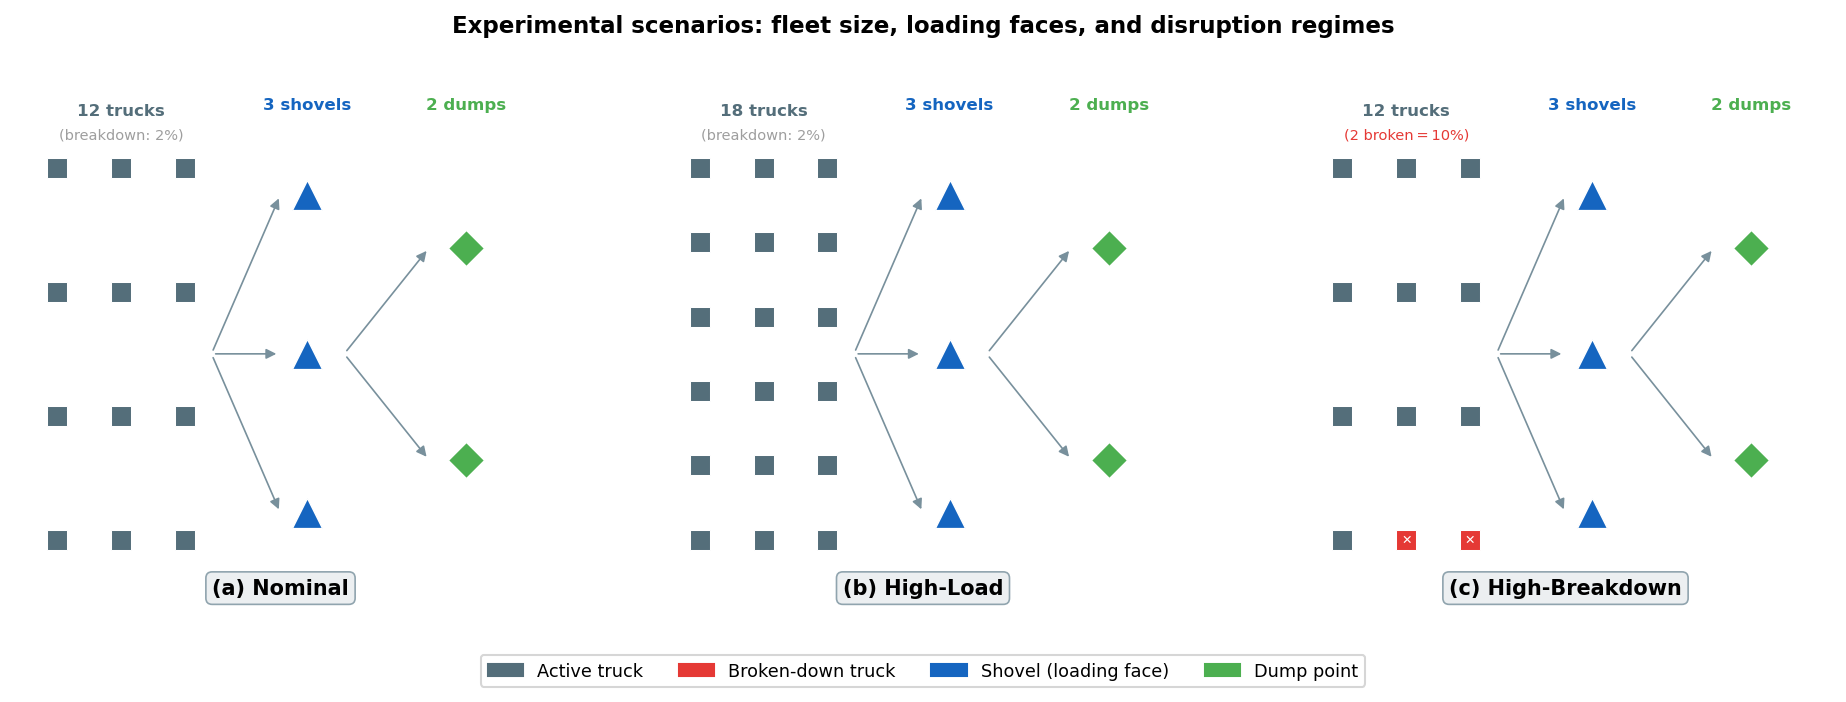
\includegraphics[width=0.95\textwidth]{figures/fig3_scenarios.png}
\caption{Configuration of the three experimental scenarios.}
\label{fig:scenarios}
\end{figure}

\subsection{Baselines}

To establish a comprehensive benchmark, the PPO agent is compared against seven other policies, grouped into three families:

\begin{itemize}
  \item \textbf{Static heuristics:} FIFO, Fixed Assignment, Nearest Shovel and Shortest Path. These represent current industrial standards.
  \item \textbf{Tabular reinforcement learning:} Q-Learning and SARSA, used to assess the impact of neural approximation relative to discrete state tables.
  \item \textbf{Value-based deep reinforcement learning:} DQN, used to contrast policy-gradient methods (PPO) with deep value-based learning.
\end{itemize}

For reproducibility, the four static heuristics are defined precisely in \cref{tab:baselines}. All of them are evaluated in exactly the same environment, with the same random seeds, as the learning agents.

\begin{table}[H]
\centering
\caption{Formal definition of the static dispatching heuristics used as baselines.}
\label{tab:baselines}
\small
\begin{tabularx}{\textwidth}{lX}
\toprule
\textbf{Policy} & \textbf{Decision rule applied when truck $i$ becomes available} \\
\midrule
FIFO             & Assign truck $i$ to the admissible shovel whose loading request has been pending for the longest time (ties broken by shovel index). \\
Fixed Assignment & Assign truck $i$ to the shovel $j(i)$ determined at the beginning of the shift; reassignment occurs only if $j(i)$ is unavailable (breakdown). \\
Nearest Shovel   & Assign truck $i$ to the admissible shovel minimising the travel distance from the current position of the truck, ignoring queue length. \\
Shortest Path    & Assign truck $i$ to the admissible destination minimising the expected travel time computed by Dijkstra's algorithm on the current road graph. \\
\bottomrule
\end{tabularx}
\end{table}

\subsection{Metrics}
\label{sec:metrics}

We use the following key performance indicators (KPIs) to assess the effectiveness of each policy:

\begin{enumerate}
  \item \textbf{Productivity:} total tonnage delivered per hour (t/h).
  \item \textbf{Average waiting time:} mean time during which trucks remain idle in queues per cycle (min).
  \item \textbf{Equipment utilisation:} percentage of time during which shovels and trucks perform productive tasks (\%).
  \item \textbf{Specific consumption:} fuel or energy consumed per tonne hauled, reflecting sustainability (L/t). Full cross-scenario values (all 8 policies $\times$ 3 scenarios) are reported in \cref{tab:efficiency} (\cref{sec:sustainability}).
  \item \textbf{Number of completed cycles:} total number of load--haul--dump cycles completed during the shift. Reported for all eight policies across all three scenarios in \cref{tab:cycles_reward} (\cref{sec:results}).
  \item \textbf{Cumulative reward:} the total reward accumulated over the episode under the reference weight vector ($w_1=1,\,w_2=0.1,\,w_3=0.05,\,w_4=0.3$). Because all policies in the main benchmark are evaluated with the same weights, the values are cross-comparable; they are reported in \cref{tab:cycles_reward}. The sensitivity of PPO's reward to $w_4$ alone is further examined in the ablation study (\cref{tab:ablation}).
  \item \textbf{Robustness ratio:} to quantify resilience, we compute the ratio between performance in disrupted scenarios and performance under nominal conditions:
  \begin{equation}
  \mathrm{RR}(p,s) = \frac{\mathrm{Performance}(p,s)}{\mathrm{Performance}(p,\mathrm{nominal})} .
  \label{eq:rr}
  \end{equation}
\end{enumerate}

\subsection{Statistical protocol}
\label{sec:proto}

In line with high-impact research standards, we do not rely on single simulation runs.

\begin{itemize}
  \item \textbf{Replications:} each policy is evaluated over 30 independent replications in order to guarantee statistical power and the validity of confidence intervals.
  \item \textbf{Random seed control:} identical random seeds are used across all policies within each replication. This ensures that every algorithm faces exactly the same sequence of stochastic events (for example, a breakdown occurs at the same minute for PPO as for FIFO).
  \item \textbf{Normality and variance:} we apply the Shapiro--Wilk test to check normality and Levene's test to assess the homogeneity of variances (homoscedasticity).
\end{itemize}

\paragraph{Inferential statistics.} Based on the outcome of the normality tests, we apply:

\begin{itemize}
  \item \textbf{One-way ANOVA} (or \textbf{Welch's ANOVA} in case of unequal variances) to determine whether significant differences exist between policies; the \textbf{Kruskal--Wallis} test is used if the normality assumption is violated.
  \item \textbf{Post-hoc tests:} pairwise Welch $t$-tests with Holm--Bonferroni correction (paired with Welch's ANOVA, as they do not assume homoscedasticity) or Dunn's rank-based test with Holm correction (paired with Kruskal--Wallis) to identify specific pairwise differences. Tukey's HSD and Games--Howell are deliberately avoided: both require homoscedasticity or a Studentized-range reference distribution that is inappropriate when the primary test is Kruskal--Wallis.
  \item \textbf{Holm--Bonferroni correction:} applied to all $p$-values in order to control type I error in multiple comparisons.
  \item \textbf{Effect size:} we compute Cohen's $d$ (or Hedges' $g$ for small samples) and Cliff's delta to measure the practical magnitude of performance improvements.
  \item \textbf{Confidence intervals:} 95\% intervals are generated using the bootstrap method to provide a robust range for mean performance.
\end{itemize}

\subsection{Reproducibility settings}

To ensure the reproducibility of this study, all simulation parameters and hyperparameters are fixed. The simulation is implemented in Python 3.11.11 using Gymnasium 1.2.3 \cite{MarkTowers2025} and Stable-Baselines3 \cite{AntoninRaffin2021}. Training of the PPO and DQN agents was carried out on a standardised hardware configuration, with all random number generators (RNG) initialised from a global seed. The specific reward weights ($w_1 = 1$, $w_2 = 0.1$, $w_3 = 0.05$, $w_4 = 0.3$) were kept constant throughout the reinforcement learning experiments. The source code, configuration files and seed lists are archived in the repository and described in the Code Availability section so that the full experimental protocol can be inspected and rerun.

\paragraph{Training and evaluation protocol.}
PPO and DQN were trained exclusively on the nominal scenario ($N=12$ trucks, breakdown rate~$=2\%$) for 2~million environment timesteps. Q-Learning and SARSA, whose natural unit of progress is the episode rather than the individual environment interaction, were trained for 30,000 episodes on the same scenario (see Table~\ref{tab:hyper}); the two budgets are not directly comparable in wall-clock terms. The deep agents converge within their budget; the tabular agents do not, so their reported performance is a lower bound rather than a converged optimum. Evaluation on the high-load and high-breakdown scenarios was subsequently performed in \textit{zero-shot} fashion: the trained agents were deployed without any additional fine-tuning, directly measuring out-of-distribution generalisation. This train-on-nominal / test-on-disrupted design is the methodological basis of the resilience claims in \cref{sec:results}: if agents had been retrained per scenario, the study would measure adaptation, not robustness.
% ============================================================================
% Section 6: Results
% ============================================================================
\section{Results}
\label{sec:results}

This section presents the empirical results obtained from our multi-scenario simulations. We focus in particular on the performance hierarchy of the evaluated policies and on the evolution of their behaviour under operational stress.

\subsection{Productivity}

The primary performance indicator, productivity in tonnes per hour, was measured across all scenarios. \cref{tab:productivity} reports mean values and standard deviations for the eight policies, together with the specific fuel consumption under high load; the full cross-scenario fuel values appear in \cref{tab:efficiency}.

\begin{table}[H]
\centering
\caption{Mean productivity (t/h), reported as mean $\pm$ standard deviation over 30 replications.}
\label{tab:productivity}
\footnotesize\setlength{\tabcolsep}{3pt}
\begin{tabularx}{\textwidth}{@{}lXXXc@{}}
\toprule
\textbf{Policy} & \textbf{Nominal (t/h)} & \textbf{High-load (t/h)} & \textbf{High-breakdown (t/h)} & \textbf{L/t} \\
\midrule
FIFO               & 3,285.92 $\pm$ 41 & 4,754.75 $\pm$ 63  & 3,117.92 $\pm$ 62 & 0.0546 \\
Fixed Assignment   & 4,071.67 $\pm$ 43 & \textbf{5,873.58 $\pm$ 76} & 3,818.50 $\pm$ 67 & \textbf{0.0444} \\
Nearest Shovel     & 3,824.92 $\pm$ 67 & 3,948.00 $\pm$ 39  & 3,661.58 $\pm$ 67 & 0.0582 \\
Shortest Path      & 3,868.08 $\pm$ 46 & 3,962.00 $\pm$ 38  & 3,692.50 $\pm$ 59 & 0.0588 \\
Q-Learning         & 3,586.33 $\pm$ 99 & 4,769.33 $\pm$ 102 & 3,180.92 $\pm$ 92 & 0.0537 \\
SARSA              & 3,085.25 $\pm$ 62 & 4,044.83 $\pm$ 76  & 2,980.83 $\pm$ 78 & 0.0612 \\
DQN (Deep RL)      & 4,134.67 $\pm$ 68 & 5,651.33 $\pm$ 74  & \textbf{3,949.17 $\pm$ 72} & 0.0445 \\
PPO (Deep RL)      & \textbf{4,176.67 $\pm$ 64} & 5,149.08 $\pm$ 325 & 3,899.58 $\pm$ 85 & 0.0475 \\
\bottomrule
\end{tabularx}
\end{table}

Under nominal conditions, PPO achieved the highest productivity (4,176.67 t/h), outperforming Fixed Assignment by 2.6\% and DQN (4,134.67 t/h) by 1.0\% (\cref{fig:productivity}). In the high-breakdown scenario, DQN proved most resilient (3,949.17 t/h), while PPO (3,899.58 t/h) fell slightly below. In the high-load scenario, Fixed Assignment dominates on raw throughput (5,873.58 t/h) and simultaneously achieves the lowest mean waiting time (43.2 min); DQN is a close second on both metrics (5,651.33 t/h, 47.8 min). The distance-based heuristics (Nearest Shovel: 3,948 t/h, 199.6 min; Shortest Path: 3,962 t/h, 204.3 min) are Pareto-dominated on both dimensions, supporting hypothesis H4. The comparatively large standard deviation of PPO under high load ($\pm$~325) reflects run-to-run variability under fleet oversaturation.

\cref{tab:cycles_reward} reports the number of completed cycles and the cumulative reward for the same runs. Because all policies are evaluated with the same weight vector, the reward values are cross-comparable. The ranking by cumulative reward matches the productivity ranking in every scenario, which confirms that the reward function effectively incentivises system-wide throughput. The sharp reward collapse of Nearest Shovel and Shortest Path under high load, 161.4 and 160.5 against more than 200 for queue-based policies, reflects the waiting-time penalty term $w_4 P_{\mathrm{wait}}$ and confirms empirically that the multi-objective reward penalises congestion.

\begin{figure}[H]
\centering
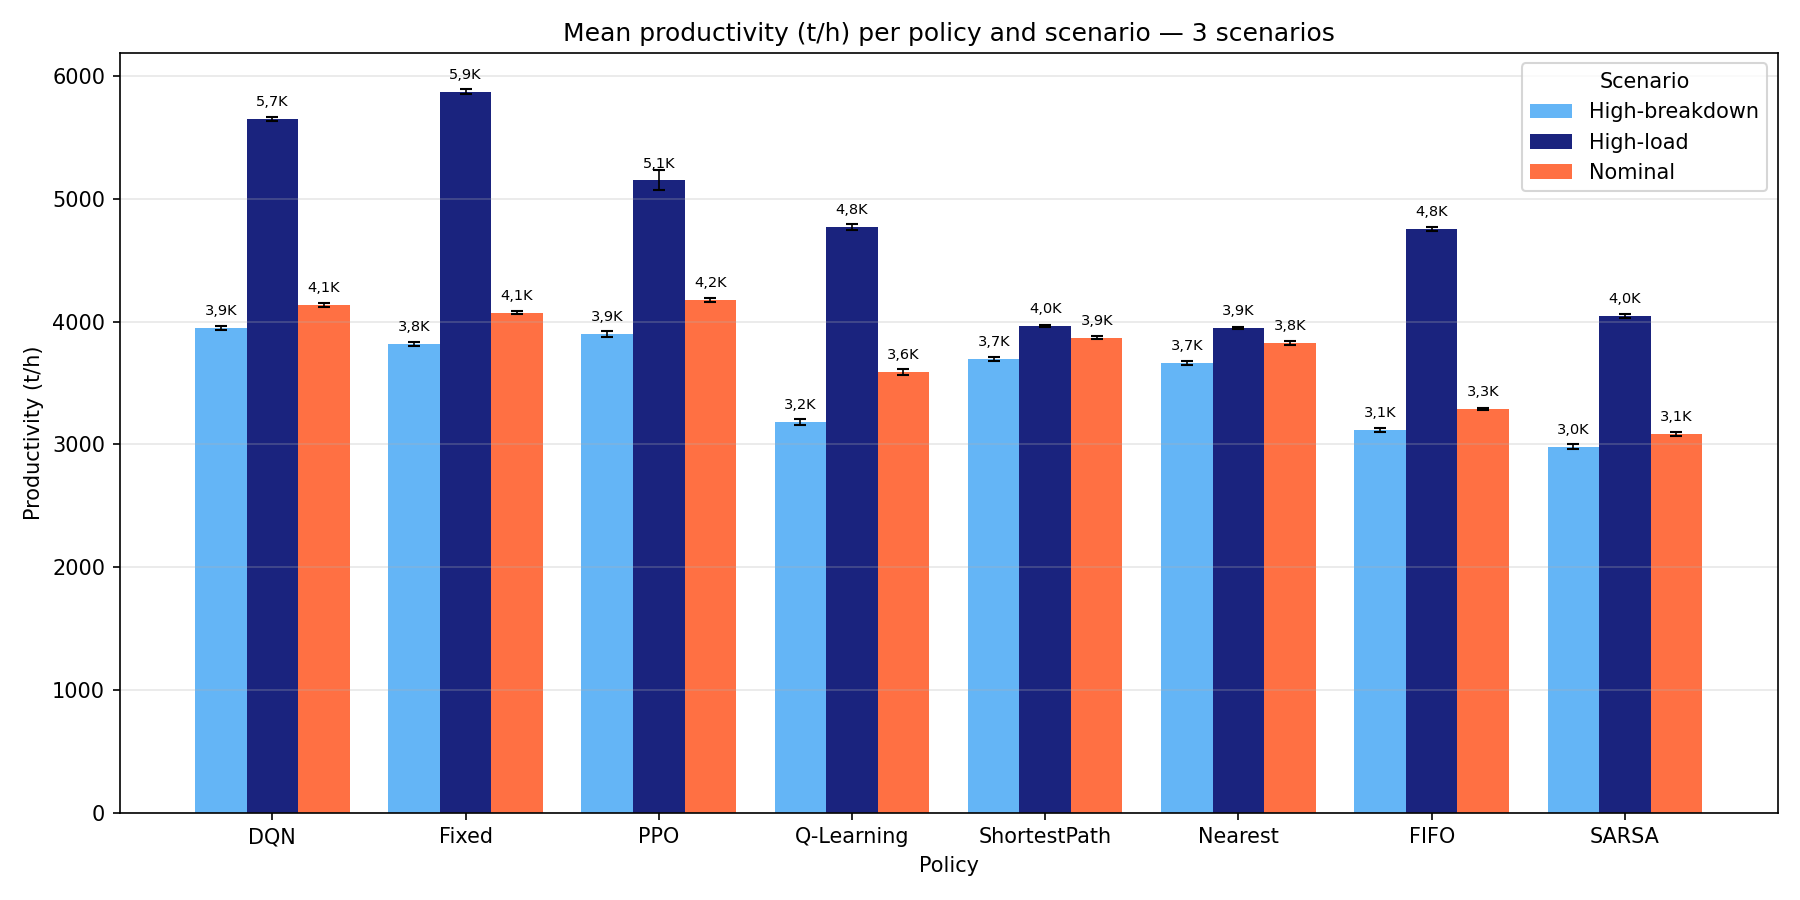
\includegraphics[width=0.92\textwidth]{figures/barplot_productivite_scenarios.png}
\caption{Mean productivity per policy and per scenario. Error bars indicate 95\% bootstrap confidence intervals over the 30 replications.}
\label{fig:productivity}
\end{figure}

\begin{table}[H]
\centering
\caption{Mean number of completed cycles and cumulative reward per policy and scenario, over 30 replications under the reference weight vector.}
\label{tab:cycles_reward}
\small
\setlength{\tabcolsep}{4pt}
\renewcommand{\arraystretch}{1.05}
\begin{tabularx}{\textwidth}{@{}l*{6}{>{\centering\arraybackslash}X}@{}}
\toprule
\multirow{2}{*}{\textbf{Policy}}
  & \multicolumn{3}{c}{\textbf{Completed cycles}}
  & \multicolumn{3}{c}{\textbf{Cumulative reward}} \\
\cmidrule(lr){2-4}\cmidrule(lr){5-7}
  & \textbf{N} & \textbf{HL} & \textbf{HB}
  & \textbf{N}   & \textbf{HL}   & \textbf{HB} \\
\midrule
FIFO              & 187.8 & 271.7 & 178.2 & 163.1 & 234.0 & 155.0 \\
Fixed Assignment  & 232.7 & \textbf{335.6} & 218.2 & 210.7 & \textbf{301.3} & 197.7 \\
Nearest Shovel    & 218.6 & 225.6 & 209.2 & 193.0 & 161.4 & 185.7 \\
Shortest Path     & 221.0 & 226.4 & 211.0 & 194.7 & 160.5 & 187.0 \\
Q-Learning        & 204.9 & 272.5 & 181.8 & 178.9 & 230.6 & 155.6 \\
SARSA             & 176.3 & 231.1 & 170.3 & 147.3 & 179.7 & 143.2 \\
DQN (Deep RL)     & 236.3 & 322.9 & \textbf{225.7} & 213.8 & 288.9 & \textbf{204.4} \\
PPO (Deep RL)     & \textbf{238.7} & 294.2 & 222.8 & \textbf{216.6} & 253.0 & 201.5 \\
\bottomrule
\end{tabularx}
\end{table}

\subsection{Waiting time and congestion}
\label{sec:waiting}

One of the key observations of this study is the decoupling between productivity and system fluidity (\cref{fig:waiting,fig:pareto}). In the high-load scenario, although productivity increases because of the sheer number of trucks, congestion becomes the limiting factor.

We observed a \textit{congestion collapse} specific to distance-based heuristics (Nearest Shovel: $199.6 \pm 8.1$ min, Shortest Path: $204.3 \pm 5.8$ min), where competing trucks saturate the same shovel simultaneously. Queue-based heuristics are more resilient: FIFO ($45.2 \pm 4.0$ min) and Fixed Assignment ($43.2 \pm 4.0$ min) manage congestion almost as effectively as DQN ($47.8 \pm 3.8$ min). PPO shows higher variance ($99.3 \pm 21.3$ min), reflecting occasional suboptimal routing decisions under extreme fleet saturation. These results indicate that the dispatching \emph{type} (distance-based vs.\ queue-based vs.\ learned) matters more than the RL/non-RL distinction for the waiting-time metric. In the high-breakdown scenario, DRL agents recover competitive fluidity (PPO: 69.9~min; DQN: 71.8~min), outperforming tabular methods (SARSA: 81.8~min; Q-Learning: 87.9~min) and distance-based heuristics ($\approx\!94$~min), though queue-based heuristics retain a moderate advantage (FIFO: 55.1~min; Fixed Assignment: 57.2~min). \cref{fig:waiting} contrasts the three policies that span the range of observed behaviours: Fixed Assignment and DQN remain below 50~min in all three scenarios, whereas PPO reaches 99.3~min under fleet oversaturation. The full eight-policy comparison appears in \cref{tab:waiting}.

\begin{table}[H]
\centering
\caption{Mean waiting time per cycle (minutes) $\pm$ standard deviation over 30 replications.}
\label{tab:waiting}
\small
\begin{tabular}{lccc}
\toprule
\textbf{Policy} & \textbf{Nominal (min)} & \textbf{High-load (min)} & \textbf{High-breakdown (min)} \\
\midrule
FIFO               & 33.5 $\pm$ 5.8  & 45.2 $\pm$ 4.0  & 55.1 $\pm$ 8.6  \\
Fixed Assignment   & \textbf{29.4 $\pm$ 4.2}  & \textbf{43.2 $\pm$ 4.0}  & 57.2 $\pm$ 7.0  \\
Nearest Shovel     & 75.1 $\pm$ 6.4  & 199.6 $\pm$ 8.1 & 93.8 $\pm$ 7.1  \\
Shortest Path      & 76.6 $\pm$ 6.1  & 204.3 $\pm$ 5.8 & 94.7 $\pm$ 6.5  \\
Q-Learning         & 58.1 $\pm$ 6.7  & 69.3 $\pm$ 3.9  & 87.9 $\pm$ 7.0  \\
SARSA              & 68.2 $\pm$ 5.8  & 119.9 $\pm$ 12.1 & 81.8 $\pm$ 8.4 \\
DQN (Deep RL)      & 43.7 $\pm$ 5.2  & 47.8 $\pm$ 3.8  & 71.8 $\pm$ 6.2  \\
PPO (Deep RL)      & 33.5 $\pm$ 4.8  & 99.3 $\pm$ 21.3 & \textbf{69.9 $\pm$ 8.0} \\
\bottomrule
\end{tabular}
\end{table}

\begin{figure}[H]
\centering
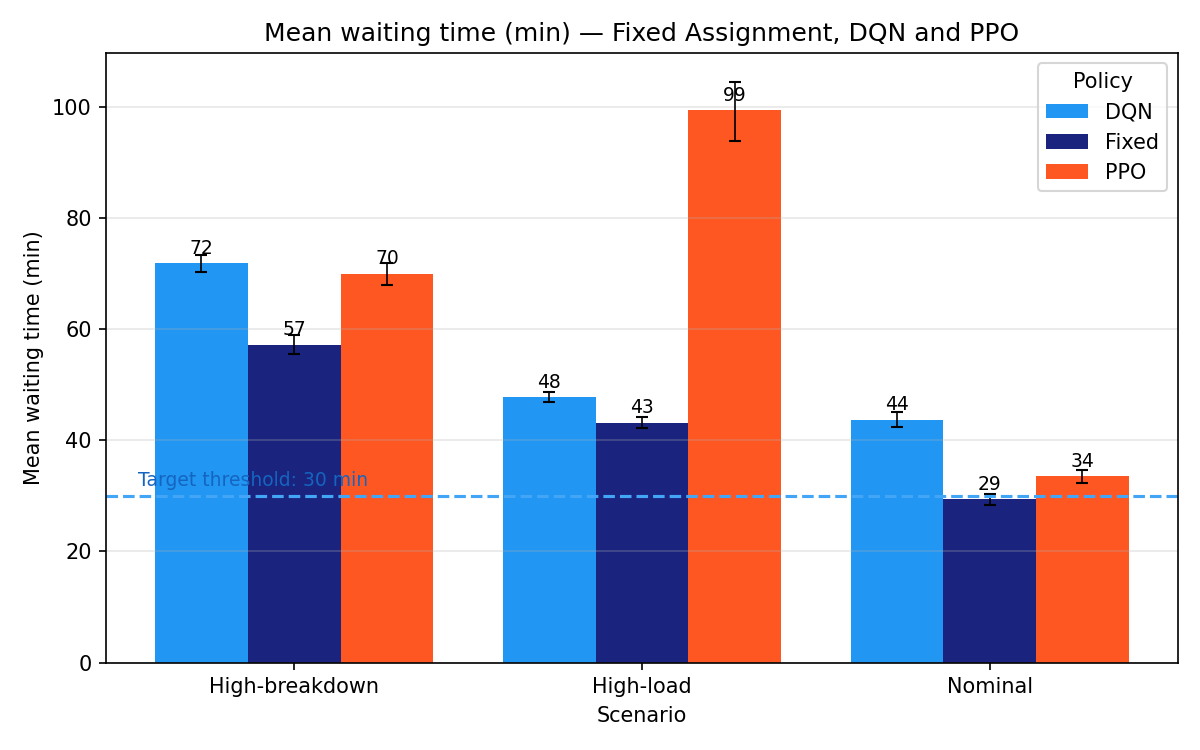
\includegraphics[width=0.92\textwidth]{figures/wait_time_comparison.png}
\caption{Mean waiting time per cycle for Fixed Assignment, DQN and PPO. Error bars indicate 95\% bootstrap confidence intervals.}
\label{fig:waiting}
\end{figure}

\cref{fig:pareto} places every (policy, scenario) pair in the productivity--waiting plane, so that the lower right corner corresponds to the most desirable behaviour. The best-performing points belong to the high-load scenario rather than to the nominal one: Fixed Assignment reaches approximately 5,900~t/h at 42~min and DQN approximately 5,600~t/h at 47~min, because the 50\% larger fleet produces higher aggregate throughput while both policies keep congestion in check. Distance-based heuristics reach approximately 200~min of waiting in the same scenario, which indicates a severe congestion regime. In the nominal scenario, PPO and Fixed Assignment form the local Pareto front, between 4,100 and 4,200~t/h for 29 to 34~min. No single policy occupies the global Pareto front across all three regimes, which confirms hypothesis~H4.

\begin{figure}[H]
\centering
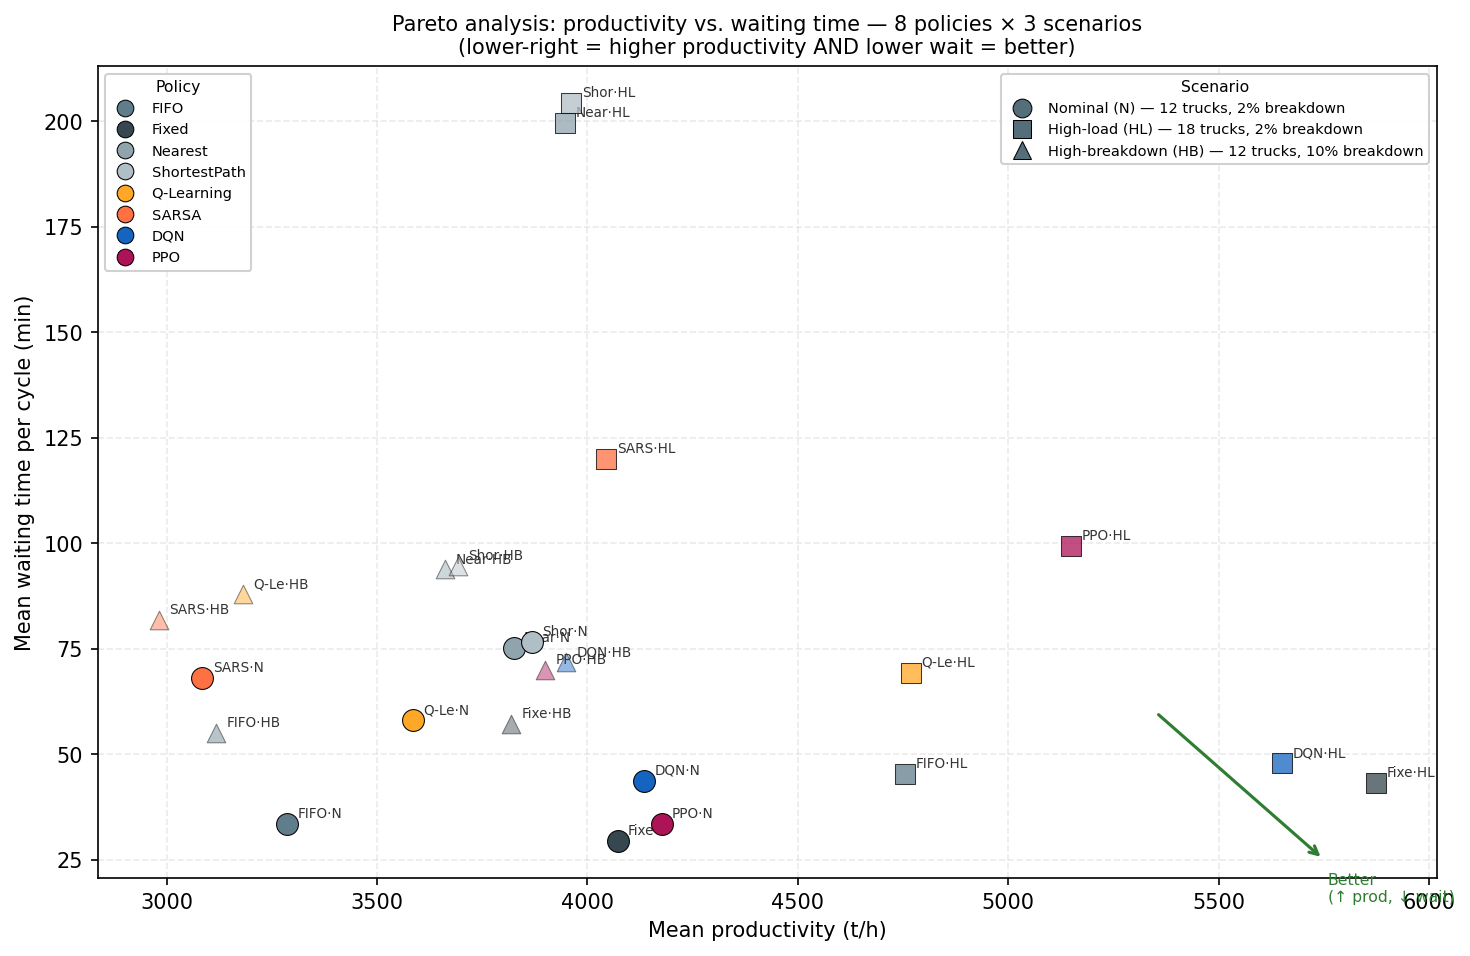
\includegraphics[width=0.88\textwidth]{figures/pareto_productivity_waiting.png}
\caption{Productivity--waiting time Pareto analysis. Colour denotes the policy and marker shape the scenario: circle for nominal, square for high-load, triangle for high-breakdown. Labels follow the ``Policy\textperiodcentered Scenario'' convention.}
\label{fig:pareto}
\end{figure}

\subsection{Robustness under disruptions}
\label{sec:robustness}

This analysis constitutes the scientific core of the present work. All RL agents were trained exclusively on the nominal scenario and evaluated in \emph{zero-shot} fashion on disrupted scenarios without any additional fine-tuning; the metrics below therefore measure out-of-distribution resilience, not adaptation capacity.

Two complementary degradation metrics are introduced alongside the robustness ratio $\mathrm{RR}$ (\cref{eq:rr}). The breakdown degradation index $\Delta_{\mathrm{breakdown}}$ quantifies the share of productivity lost when moving from nominal to high-breakdown conditions:

\begin{equation}
\Delta_{\mathrm{breakdown}} = \frac{P_{\mathrm{nominal}} - P_{\mathrm{breakdown}}}{P_{\mathrm{nominal}}} \times 100 .
\label{eq:delta}
\end{equation}

\noindent The waiting-time increase index $\Delta_{\mathrm{wait}}^{s}$ captures queue degradation in disrupted scenario $s$ relative to nominal:

\begin{equation}
\Delta_{\mathrm{wait}}^{s} = \frac{W_{s} - W_{\mathrm{nominal}}}{W_{\mathrm{nominal}}} \times 100 .
\label{eq:delta_wait}
\end{equation}

\noindent Together these two indices provide a two-dimensional resilience profile: one dimension captures the ability to sustain throughput; the other captures the ability to contain queue formation under stress. \cref{tab:robustness} reports the productivity robustness ratio $\mathrm{RR}$, the throughput degradation $\Delta_{\mathrm{breakdown}}$ of \cref{eq:delta}, and the waiting-time increase of \cref{eq:delta_wait} measured under high load and under high breakdown, both relative to the nominal scenario.

\begin{table}[H]
\centering
\caption{Multi-dimensional robustness analysis for all policies. Lower degradation values indicate higher resilience.}
\label{tab:robustness}
\small
\setlength{\tabcolsep}{4.5pt}
\begin{tabular}{l r r r r r}
\toprule
 & \multicolumn{2}{c}{\textbf{Productivity RR}} & \textbf{} & \multicolumn{2}{c}{\textbf{Waiting-time increase (\%)}} \\
\cmidrule(lr){2-3}\cmidrule(lr){5-6}
\textbf{Policy} & \textbf{RR(HL)} & \textbf{RR(HB)} & \textbf{$\Delta_{\mathrm{breakdown}}$ (\%)} & \textbf{$\Delta_{\mathrm{wait}}^{\mathrm{HL}}$} & \textbf{$\Delta_{\mathrm{wait}}^{\mathrm{HB}}$} \\
\midrule
FIFO               & 1.447 & 0.949 &  5.11  & +35.0  & +64.5  \\
Fixed Assignment   & 1.443 & 0.938 &  6.22  & +47.0  & +94.8  \\
Nearest Shovel     & 1.032 & 0.957 &  4.27  & +165.9 & +24.9  \\
Shortest Path      & 1.024 & 0.955 &  4.54  & +166.7 & +23.6  \\
Q-Learning         & 1.330 & 0.887 & 11.30  & +19.4  & +51.3  \\
SARSA              & 1.311 & \textbf{0.966} & \textbf{3.38} & +75.9 & \textbf{+20.0} \\
DQN (Deep RL)      & 1.367 & 0.955 &  4.49  & \textbf{+9.3}  & +64.3  \\
PPO (Deep RL)      & 1.233 & 0.934 &  6.63  & +196.4 & +108.7 \\
\bottomrule
\end{tabular}
\end{table}

\noindent\textbf{Throughput degradation under equipment failures.} On the productivity axis, the breakdown-degradation ordering is counterintuitive. The highest \emph{relative} stability is shown by SARSA ($\mathrm{RR}_{\mathrm{HB}}=0.966$, $\Delta=3.38\%$) and the distance-based heuristics (4.27\% and 4.54\%), but this reflects their already-compressed nominal baselines rather than genuine resilience. The policy that delivers the highest \emph{absolute} throughput under breakdown is DQN (3,949.17~t/h, $\Delta=4.49\%$). PPO ($\Delta=6.63\%$) degrades more than both DQN and FIFO (5.11\%), suggesting that its nominal-trained policy does not fully transfer to disrupted dynamics. Q-Learning shows the largest productivity collapse ($\Delta=11.30\%$), confirming that tabular value functions do not generalise across discrete failure shocks.

\noindent\textbf{Queue degradation under fleet congestion.} The waiting-time dimension reveals the most striking result of this study. Under high-load, DQN's waiting time increases by only $\Delta_{\mathrm{wait}}^{\mathrm{HL}}=+9.3\%$, the most resilient policy by a wide margin. PPO's waiting time increases by $+196.4\%$, the largest growth of any policy despite its nominal dominance. Distance-based heuristics also collapse: Nearest Shovel ($+165.9\%$) and Shortest Path ($+166.7\%$) cannot resolve competing claims on loaded shovels once the fleet exceeds absorption capacity (see \cref{sec:waiting}). Queue-based heuristics (FIFO $+35.0\%$, Fixed Assignment $+47.0\%$) and Q-Learning ($+19.4\%$) remain relatively contained. Under high-breakdown, SARSA again leads on the waiting-time dimension ($+20.0\%$), followed by Nearest and Shortest Path ($+24.9\%$, $+23.6\%$); PPO records the largest absolute queue growth ($+108.7\%$), exceeding even Fixed Assignment ($+94.8\%$).

\medskip
\noindent\textbf{Core finding: decoupling of nominal efficiency from operational resilience.} \cref{tab:robustness} reveals a systematic inversion of the performance hierarchy across regimes. PPO, the top-performing policy under nominal conditions (4,176.67~t/h, 33.51~min waiting), is among the most vulnerable under both congestion ($+196\%$ waiting-time increase) and breakdown ($\Delta=6.63\%$). DQN, ranked second nominally, delivers the best absolute breakdown throughput and the most contained congestion response (+9.3\%). This reversal demonstrates that nominal productivity is a poor predictor of operational resilience, and that single-regime evaluation would have led to the incorrect conclusion that PPO is the most deployable policy in variable mining environments. In \cref{fig:heatmap}, the upper block reports the productivity change relative to nominal and the lower block the waiting-time change, the latter on a negated scale so that a degradation appears as a negative value in both blocks. The sharpest contrast appears in the high-load column, where the waiting time of PPO grows by 196\% while DQN remains stable at 9\%.

\begin{figure}[H]
\centering
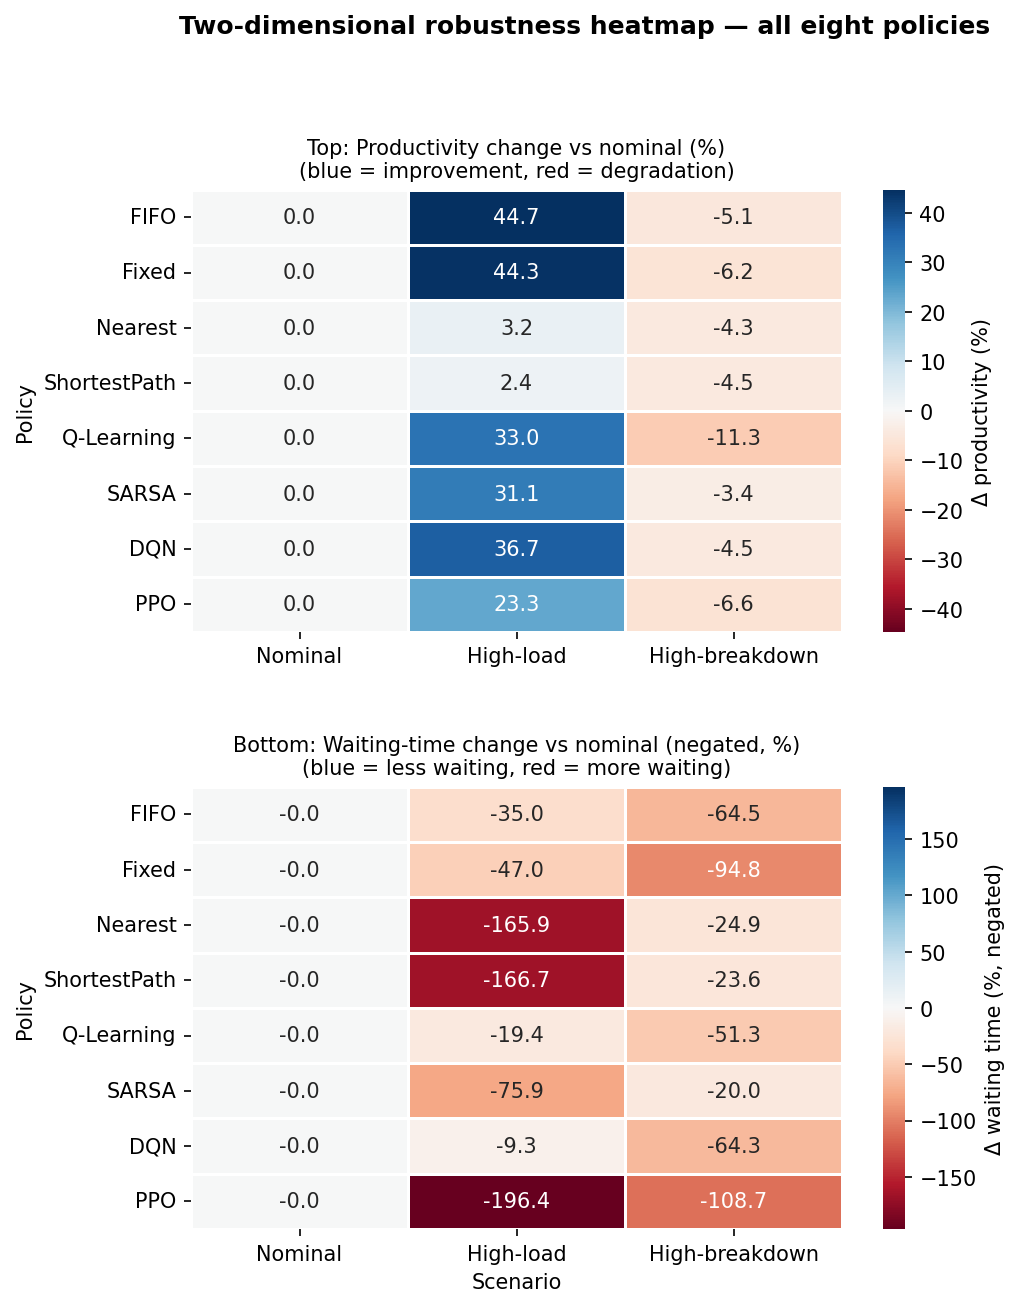
\includegraphics[width=0.9\textwidth]{figures/robustness_heatmap.png}
\caption{Robustness heatmap for the eight policies across the three scenarios. Blue denotes an improvement relative to nominal and red a degradation; the waiting-time block is plotted on a negated scale so that both blocks share the same reading direction.}
\label{fig:heatmap}
\end{figure}

\subsection{Statistical significance}

The choice of test follows the distributional diagnostics. Under nominal conditions, Shapiro--Wilk rejects normality in six of the eight groups and Levene detects heterogeneous variances ($p=2.3\times10^{-8}$); with $n=30$ per group the Welch $t$-test remains valid under the central limit theorem, so a Welch Analysis of Variance is used as the omnibus test and pairwise Welch $t$-tests with Holm correction as the post-hoc criterion. In the two disrupted scenarios, at least one group violates normality and the variances are heterogeneous, so Kruskal--Wallis is used as the omnibus test with Dunn's rank-based post-hoc test as the primary pairwise criterion. All three omnibus tests reveal a significant effect of the dispatching policy on productivity ($p<0.001$).

Dunn's test is conservative under many-group correction and does not detect a significant difference at $\alpha=0.05$ for three comparisons. The corresponding Welch $t$-tests yield $p=5.2\times10^{-8}$ for Fixed Assignment against DQN under high load, $p=2.7\times10^{-8}$ for PPO against Fixed Assignment under high breakdown, and $p=5.4\times10^{-4}$ for DQN against PPO in the same scenario. These parametric results are reported for completeness; the Dunn post-hoc remains the primary criterion, consistent with the Kruskal--Wallis framework. Effect sizes and 95\% confidence intervals of the mean differences are derived from pairwise Welch $t$-tests in all scenarios. \cref{tab:stats} reports the full pairwise post-hoc results.

\begin{itemize}
  \item \textbf{Nominal pairwise comparisons (Welch):} PPO $>$ Fixed Assignment ($p=4.01\times10^{-18}$, $d=1.942$, large); DQN $>$ Fixed Assignment ($p=2.13\times10^{-8}$, $d=1.112$, large); PPO $>$ DQN ($p=3.21\times10^{-4}$, $d=0.640$, medium).
  \item \textbf{High-load (Kruskal--Wallis, Dunn post-hoc):} Fixed Assignment leads PPO ($p=1.27\times10^{-5}$, $d=3.096$, large) and DQN ($p=0.062$, $d=3.004$; borderline non-significant after Holm correction). DRL policies do not outperform the static heuristic on raw throughput in this regime; the advantage of Fixed Assignment over DQN is numerically large but does not clear the corrected threshold.
  \item \textbf{High-breakdown (Kruskal--Wallis, Dunn post-hoc):} DQN $>$ Fixed Assignment ($p=5.78\times10^{-3}$, $d=1.896$, large). PPO leads Fixed Assignment by 81~t/h ($d=1.065$) but the rank-based post-hoc does not reach significance ($p=0.144$); the corresponding Welch $t$-test yields $p=2.7\times10^{-8}$, suggesting the difference is real but attenuated by the conservativeness of the many-group rank correction. DQN leads PPO by 49.6~t/h ($d=0.636$, Dunn $p=0.686$, Welch $p=5.4\times10^{-4}$); on balance, DQN is the dominant deep-RL policy under breakdown conditions.
\end{itemize}

\begin{table}[H]
\centering
\caption{Summary of statistical tests on productivity (Holm--Bonferroni corrected $p$-values).}
\label{tab:stats}
\scriptsize
\setlength{\tabcolsep}{3pt}
\begin{tabular}{llccc}
\toprule
\textbf{Scenario} & \textbf{Comparison} & \textbf{$p$-value} & \textbf{Effect size (Cohen's $d$)} & \textbf{95\% CI of difference} \\
\midrule
Nominal        & Welch ANOVA (global)      & $p < 0.001$, $F=3339$ & n/a & n/a \\
Nominal        & PPO vs Fixed Assmt (Welch)  & $p=4.01\times10^{-18}$ & $d=1.942$ & $[85.4,\;124.6]$ \\
Nominal        & DQN vs Fixed Assmt (Welch)  & $p=2.13\times10^{-8}$ & $d=1.112$ & $[42.5,\;\;\;83.5]$ \\
Nominal        & PPO vs DQN (Welch)          & $p=3.21\times10^{-4}$ & $d=0.640$ & $[18.3,\;\;\;65.7]$ \\
High-load      & Kruskal--Wallis              & $p < 0.001$, $H=445$            & n/a & n/a \\
High-load      & Fixed vs DQN (Dunn)          & $p = 0.062$                     & $d=3.004$ & $[183.5,\;261.0]$ \\
High-load      & Fixed vs PPO (Dunn)                & $p = 1.27\times10^{-5}$         & $d=3.096$ & $[600.4,\;848.6]$ \\
High-breakdown & Kruskal--Wallis              & $p < 0.001$, $H=437$            & n/a & n/a \\
High-breakdown & DQN vs Fixed (Dunn)                & $p = 5.78\times10^{-3}$         & $d=1.896$ & $[105.7,\;155.6]$ \\
High-breakdown & PPO vs Fixed (Dunn)          & $p = 0.144$                     & $d=1.065$ & $[53.5,\;108.6]$ \\
High-breakdown & DQN vs PPO (Dunn)            & $p = 0.686$                     & $d=0.636$ & $[21.4,\;\;\;77.8]$ \\
\bottomrule
\end{tabular}
\end{table}

\subsection{Inter-replication stability}
\label{sec:stability}

Beyond mean performance, a policy is only deployable if its behaviour is reproducible from one shift to the next. We therefore compute the coefficient of variation (CV\,=\,SD/mean) of productivity across the 30 replications for each policy and scenario. Shortest Path records the lowest mean CV across the three scenarios (1.25\%), although its absolute performance is among the lowest, followed by Fixed Assignment (1.37\%), FIFO and Nearest Shovel (1.52\% each). DQN is the most stable learning agent (1.59\%). By contrast, PPO exhibits the highest variability (3.34\%), driven almost entirely by its high-load replications (CV\,=\,6.31\%, SD\,=\,$\pm$\,325~t/h), where run-to-run sensitivity to routing decisions under fleet saturation is pronounced. Tabular methods also show elevated variability (Q-Learning: 2.60\%, SARSA: 2.17\%), reflecting the sensitivity of discretised value functions to stochastic events. Taken together with the productivity ranking, Fixed Assignment and DQN offer the best combination of high performance and low inter-replication variance, which makes them the most predictable policies for operational deployment.

\subsection{Convergence}

The training curves of the four reinforcement learning agents, shown in \cref{fig:convergence}, reveal distinct learning behaviours. Each curve represents a single representative training run smoothed with a moving average. Because full multi-seed training at 2~million timesteps per agent is computationally prohibitive, confidence bands on the training trajectories are not reported here; the statistical robustness of the final performance estimates is instead established by the 30-replication evaluation protocol described in \cref{sec:proto} and reflected in the confidence intervals of \cref{tab:productivity}.

\begin{itemize}
  \item \textbf{Deep RL agents:} PPO and DQN display stable convergence within 2~million steps. PPO's productivity increases monotonically and reaches a plateau around 4,000--4,200~t/h; DQN exhibits larger early oscillations attributable to its $\varepsilon$-greedy exploration, before stabilising at a similar level. The variance of the reward signal decreases progressively as training proceeds, indicating that both agents identify robust assignment strategies.
  \item \textbf{Tabular agents:} the two tabular agents behave differently over the 30,000-episode budget. Q-Learning remains flat for roughly 12,000 episodes, then improves steadily until the end of the budget without reaching a plateau, so its reported performance should be read as a lower bound on what the method could attain with a longer budget. SARSA shows no measurable improvement over the same budget, which is consistent with its low final productivity (3,085~t/h in nominal, \cref{tab:productivity}). Both outcomes indicate that a discrete representation with $n_{\text{bins}}=8$ per dimension cannot capture the high-dimensional interdependencies of a 12-truck multi-shovel environment within a practical episode budget.
\end{itemize}

Deep and tabular agents are plotted on separate panels in \cref{fig:convergence} because they are recorded on different quantities: the deep agents on productivity in tonnes per hour, the tabular agents on cumulative episode reward. The panels are therefore not directly comparable in magnitude, and only the shape of each trajectory should be read across them.

\begin{figure}[H]
\centering
\begin{subfigure}[b]{0.49\textwidth}
  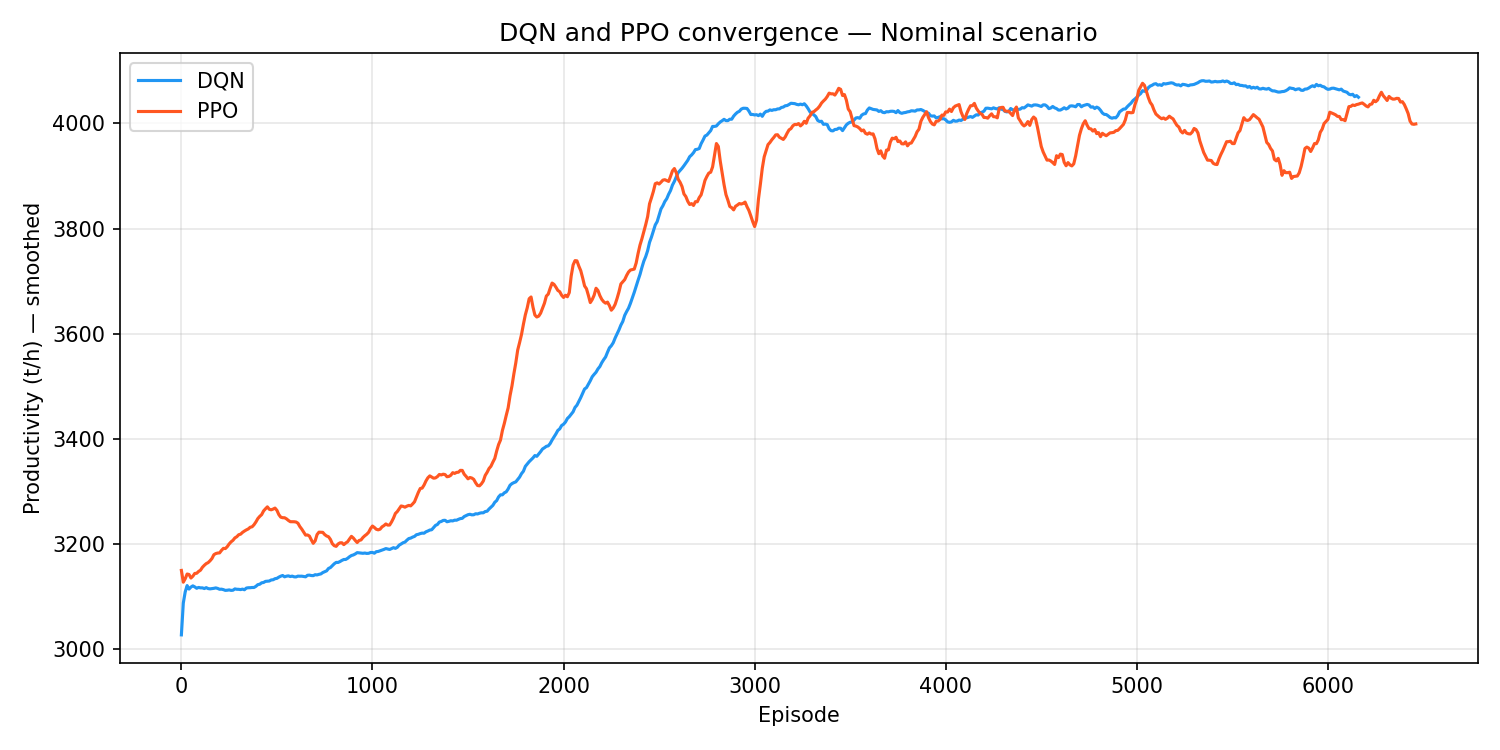
\includegraphics[width=\textwidth]{figures/learning_curves_deeprl_nominal.png}
  \caption{Deep RL agents (DQN, PPO), nominal scenario}
\end{subfigure}
\hfill
\begin{subfigure}[b]{0.49\textwidth}
  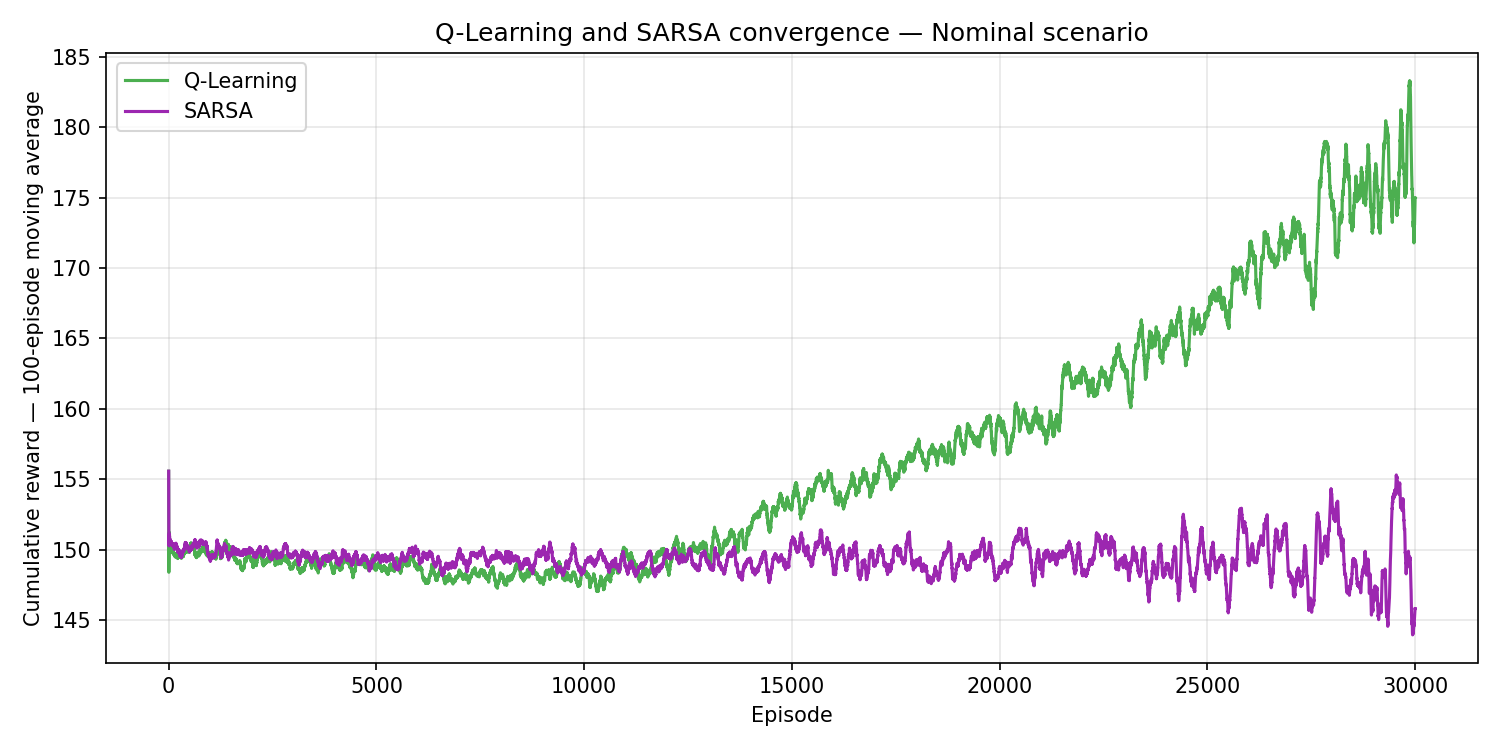
\includegraphics[width=\textwidth]{figures/learning_curves_nominal.png}
  \caption{Tabular agents (Q-Learning, SARSA), nominal scenario}
\end{subfigure}
\caption{Training curves on the nominal scenario, single representative run. Left: productivity of the deep agents in tonnes per hour. Right: cumulative episode reward of the tabular agents, 100-episode moving average.}
\label{fig:convergence}
\end{figure}

\subsection{Ablation study}
\label{sec:ablation}

The ablation study focuses on the weight of the waiting-time penalty ($w_4$) in the reward function, all other weights being held constant ($w_1 = 1$, $w_2 = 0.1$, $w_3 = 0.05$). For each value of $w_4$, a single PPO model was trained from scratch; the reported mean and standard deviation are computed over 30 independent evaluation episodes of that trained model, each with a different random seed. The standard deviation therefore reflects evaluation variability under simulation stochasticity rather than training variance; conclusions about training stability would require multiple independent training runs.

The results reveal a non-monotonic relationship between $w_4$ and performance. When $w_4 = 0$, the agent achieves 4,160.9~t/h with 41.5~min waiting time: productivity is marginally lower than the reference ($-0.4\%$) but wait times increase by 23.9\%. The surprising finding is at $w_4 = 0.1$: a small but non-zero penalty yields the \emph{worst} results on both metrics simultaneously (3,931.7~t/h, $-5.9\%$; 74.8~min, $+123\%$). This suggests that an insufficiently weighted penalty introduces conflicting gradient signals during training, causing the policy to converge to a suboptimal equilibrium rather than a coherent strategy. At $w_4 = 0.3$, the agent achieves the best trade-off (4,176.7~t/h, 33.5~min), confirming that a well-calibrated wait penalty guides the policy toward system-wide flow without sacrificing throughput. With $w_4 = 0.5$, an overly conservative penalty reverses the gain: productivity collapses to 3,683.8~t/h ($-11.8\%$), waiting time rises to 79.3~min ($+137\%$), and equipment utilisation falls to 83.7\%, the lowest across all configurations. The notably larger standard deviation ($\pm$~158~t/h) reflects higher evaluation variance under this configuration, suggesting the trained policy produces inconsistent routing decisions across the stochastic simulation runs. These results underline the sensitivity of reward engineering in multi-objective reinforcement learning: the choice of $w_4$ is not a simple dial, but a critical design parameter with non-monotonic effects on policy convergence; an intermediate, well-calibrated value ($w_4 = 0.3$) is essential to achieve coherent system-wide optimisation. In \cref{tab:ablation}, each row is evaluated with its own value of $w_4$, so the cumulative reward column is not directly comparable across rows.

\begin{table}[H]
\centering
\caption{Ablation study on the waiting-time penalty weight $w_4$, nominal scenario. Values are reported as mean $\pm$ standard deviation over 30 evaluation runs; each row is scored with its own $w_4$, so the reward column is not comparable across rows.}
\label{tab:ablation}
\small
\begin{tabular}{lcccc}
\toprule
\textbf{$w_4$} & \textbf{Productivity (t/h)} & \textbf{Waiting time (min)} & \textbf{Utilisation (\%)} & \textbf{Cum.\ reward} \\
\midrule
0.0  & 4{,}160.9 $\pm$ 64 & 41.5 $\pm$ 4.8 & 94.3 & 218.4 \\
0.1  & 3{,}931.7 $\pm$ 52 & 74.8 $\pm$ 4.6 & 84.5 & 205.1 \\
0.3 (ref.) & \textbf{4{,}176.7 $\pm$ 64} & \textbf{33.5 $\pm$ 4.8} & \textbf{94.5} & 216.6 \\
0.5  & 3{,}683.8 $\pm$ 158 & 79.3 $\pm$ 20.3 & 83.7 & 178.9 \\
\bottomrule
\end{tabular}

\end{table}

\paragraph{Hyperparameter sensitivity.}
The reference PPO configuration ($\alpha = 3 \times 10^{-4}$,
$c_H = 0.02$, $\varepsilon_{\text{clip}} = 0.2$,
$n_{\text{steps}} = 1024$, $n_{\text{epochs}} = 10$) follows the
canonical settings of~\cite{JohnSchulman2017}.
A preliminary qualitative sensitivity sweep was conducted prior to the final configuration:
(i)~varying the entropy coefficient over $c_H \in \{0.0,\, 0.01,\, 0.02,\, 0.05\}$
indicated that $c_H = 0.02$ provided the best observed convergence trade-off, since lower values produced premature convergence to locally optimal dispatch routes,
while higher values delayed convergence without a visible improvement in final productivity;
(ii)~learning rates outside $[10^{-4},\, 10^{-3}]$ caused either slow convergence
or oscillating reward curves;
(iii)~the clip range $\varepsilon_{\text{clip}} = 0.2$ is the canonical default~\cite{JohnSchulman2017}
and appeared insensitive in this discrete-action setting.
These qualitative observations support the chosen configuration as a reasonable starting point; a formal grid-search report is left for future work.

% ============================================================================
% Section 7: Discussion
% ============================================================================
\section{Discussion}
\label{sec:discussion}

This section interprets the experimental findings with respect to the research questions and to the regime dependence of the policy ranking. It discusses the reversal between nominal efficiency and operational resilience, the congestion mechanism specific to distance-based rules, the industrial implications of these results and the limitations of the study.

The experiments answer RQ1 by showing that no single policy achieves the highest productivity in every scenario. PPO leads under nominal conditions (4,176.7~t/h), Fixed Assignment under fleet oversaturation (5,873.6~t/h) and DQN under frequent equipment failures (3,949.2~t/h). The ranking is therefore not a property of the algorithm family but of the interaction between the dispatching logic and the operating regime, which is the central finding of this study.

Regarding RQ2, the trade-off between productivity and waiting time is itself regime-dependent. Under nominal conditions the two objectives are broadly aligned: the policies that move the most material also queue the least, and PPO and Fixed Assignment form a local Pareto front. Under fleet oversaturation the two objectives separate sharply, since Nearest Shovel and Shortest Path combine the lowest throughput with waiting times near 200~min, whereas Fixed Assignment and DQN improve on both dimensions simultaneously. The decoupling is thus not a general property of dispatching, but a consequence of how a given rule resolves competing claims once demand exceeds loading capacity.

For RQ3, the observed gaps survive correction unevenly. Under nominal conditions all three pairwise comparisons of interest remain significant after Holm correction, with large effect sizes. In the two disrupted scenarios the rank-based Dunn post-hoc is markedly more conservative: the advantage of Fixed Assignment over DQN under high load ($p=0.062$) and that of DQN over PPO under high breakdown ($p=0.686$) do not clear the threshold, although the corresponding Welch tests and the effect sizes point to a real difference. Reporting only the parametric results would therefore have overstated the evidence, which is why the Dunn post-hoc is retained as the primary criterion.

RQ4 receives a qualified answer. Deep agents do not degrade uniformly less than static rules when deployed on regimes they were not trained on. On throughput, PPO loses 6.63\% under breakdown, more than FIFO (5.11\%) and more than DQN (4.49\%). On queue formation, DQN is the most resilient policy of the benchmark under fleet oversaturation ($+9.3\%$), whereas PPO records the largest deterioration of any policy ($+196.4\%$). Zero-shot robustness is therefore a property of the individual agent rather than of the deep reinforcement learning family as a whole, and it does not follow from nominal performance.

RQ5 separates mean performance from predictability. Fixed Assignment and DQN combine high throughput with low inter-replication variance, whereas PPO is the least predictable policy of the benchmark, almost entirely because of its behaviour under fleet oversaturation. For an operator, a policy whose output fluctuates by more than six percent between shifts is harder to plan around than a slightly less productive but steadier alternative, which is a practical argument that mean productivity alone does not capture.

RQ6 shows that the ranking on specific fuel consumption does not follow the productivity ranking. DQN, second on nominal throughput, achieves the lowest consumption per tonne in two of the three scenarios, while PPO, first on nominal throughput, consumes more than Fixed Assignment under fleet oversaturation. Energy efficiency is therefore a third dimension alongside throughput and fluidity, and it reorders the policies once more.

\cref{tab:hypotheses} summarises the validation status of the four hypotheses stated in \cref{sec:rq}.

\begin{table}[H]
\caption{Validation of the four research hypotheses against empirical results.}
\label{tab:hypotheses}
\footnotesize\setlength{\tabcolsep}{4pt}
\begin{tabularx}{\textwidth}{@{}lXXl@{}}
\toprule
\textbf{Hyp.} & \textbf{Claim} & \textbf{Key evidence} & \textbf{Verdict} \\
\midrule
H1 & DRL $>$ heuristics in productivity under nominal conditions. & PPO leads nominal (4,176.7~t/h, $+2.6\%$ vs Fixed Assignment, $p<0.001$, $d=1.94$); DQN second (4,134.7~t/h, $+1.6\%$ vs Fixed, $p<0.001$, $d=1.11$). Both DRL agents outperform all four static heuristics. & \textbf{Validated} \\[4pt]
H2 & DRL shows lower degradation under disruptions. & On tonnage: PPO $\Delta{=}6.63\%$ vs FIFO $5.11\%$, which \textit{rejects} the claim (DRL degrades more). On waiting time: in high-load, DQN (47.8 min) and Q-Learning (69.3 min) outperform distance-based heuristics (Nearest 199.6, SP 204.3 min); queue-based heuristics (FIFO 45.2, Fixed 43.2 min) comparable to DQN. In high-breakdown, deep RL (PPO 69.9 min, DQN 71.8 min) also outperforms tabular RL (SARSA 81.8, Q-Learning 87.9) and distance-based heuristics ($\approx$94 min), but not queue-based heuristics (FIFO 55.1, Fixed 57.2 min). & Partially validated \\[4pt]
H3 & No single policy dominates across all regimes. & PPO best nominal; DQN best high-breakdown; Fixed Assmt best high-load (raw tonnage and fluidity simultaneously). & \textbf{Validated} \\[4pt]
H4 & High productivity $\not\Rightarrow$ low congestion. & Nearest Shovel and Shortest Path exhibit the decoupling: low productivity ($\approx$3,950 t/h) AND severe congestion ($\approx$200 min: Nearest 199.6, SP 204.3), dominated on both metrics by Fixed Assmt (5,874 t/h, 43.2 min) and DQN (5,651 t/h, 47.8 min). Dispatching \emph{type} (distance-based vs queue-based vs learned) determines the productivity--fluidity outcome. & \textbf{Validated} \\
\bottomrule
\end{tabularx}
\end{table}

\subsection{Scientific interpretation}

One of the main conclusions of this research is that no dispatching policy is universally dominant.

\begin{itemize}
  \item \textbf{PPO vs DQN:} the superiority of PPO under nominal conditions (4,176.67 t/h vs DQN 4,135 t/h, $d=0.640$) can be attributed to its policy-gradient nature, which allows smoother exploration in high-dimensional state spaces. DQN achieves the best absolute throughput under high-breakdown (3,949 t/h), leading PPO by 49.6~t/h ($d=0.636$, 95\,\% CI $[21.4,\,77.8]$~t/h; Welch $p=5.4\times10^{-4}$, Dunn post-hoc $p=0.686$). DQN's experience replay buffer allows the agent to reuse transition states involving equipment failures across multiple gradient updates, which may contribute to its robustness under breakdown conditions, a mechanism unavailable to the on-policy PPO agent.
  \item \textbf{DRL as a real-time load-steering agent:} distance-based heuristics such as Nearest Shovel create ``hot spots'' by routing every available truck to the physically closest excavator, regardless of its current queue state. Under fleet oversaturation this produces a congestion cascade: Nearest Shovel reaches 199.6~min mean waiting time in high-load vs 43.2~min for Fixed Assignment (\cref{tab:waiting}). DRL agents avoid this by learning to balance queue pressure across shovels at each decision point. \cref{fig:behavioral} provides direct empirical evidence: panel~(C) compares the assignment-entropy of Nearest Shovel and PPO over a 480-min high-load episode. Nearest Shovel's entropy collapses to $H\approx 0$ within the first cycles. All 18 trucks converge on the same geographically closest excavator, leaving the other two idle and creating the persistent hot-spot visible in panel~(A). PPO, by contrast, maintains a higher and more stable entropy, distributing traffic across all three shovels (panel~B). This broader allocation halves the mean queue backlog, which indicates that the PPO waiting-time advantage in high-load (99.3~min vs 199.6~min for Nearest Shovel, a 50\% reduction) is driven by the entropy difference rather than by a fortuitous parameter choice.
  \item \textbf{Decoupling of nominal efficiency and operational resilience:} \cref{tab:robustness} quantifies a systematic inversion of the performance hierarchy across operational regimes. PPO, the top-performing policy on nominal productivity (4,176.67~t/h), records the largest waiting-time deterioration under fleet congestion ($\Delta_{\mathrm{wait}}^{\mathrm{HL}}=+196.4\%$) and a throughput degradation ($\Delta=6.63\%$) that exceeds that of FIFO ($5.11\%$) and DQN ($4.49\%$) under high-breakdown. DQN exhibits the opposite profile: second on nominal productivity, best absolute breakdown throughput (3,949.17~t/h), and most resilient to congestion ($\Delta_{\mathrm{wait}}^{\mathrm{HL}}=+9.3\%$). This finding has a direct methodological implication: an evaluation conducted on the nominal scenario alone would rank PPO as the most deployable policy, whereas a multi-regime assessment reveals that DQN provides superior operational resilience in the two disrupted regimes. Mining FMS benchmarks should therefore be assessed across at least two contrasting disruption types before operational recommendations are made.
  \item \textbf{A multi-objective, stochastic problem:} the decoupling between tonnage and waiting time observed in the high-load scenario supports hypothesis H4 and confirms that mine dispatching should be treated as a genuinely multi-objective and stochastic decision problem rather than as a single-criterion throughput maximisation.
\end{itemize}

\begin{figure}[H]
\centering
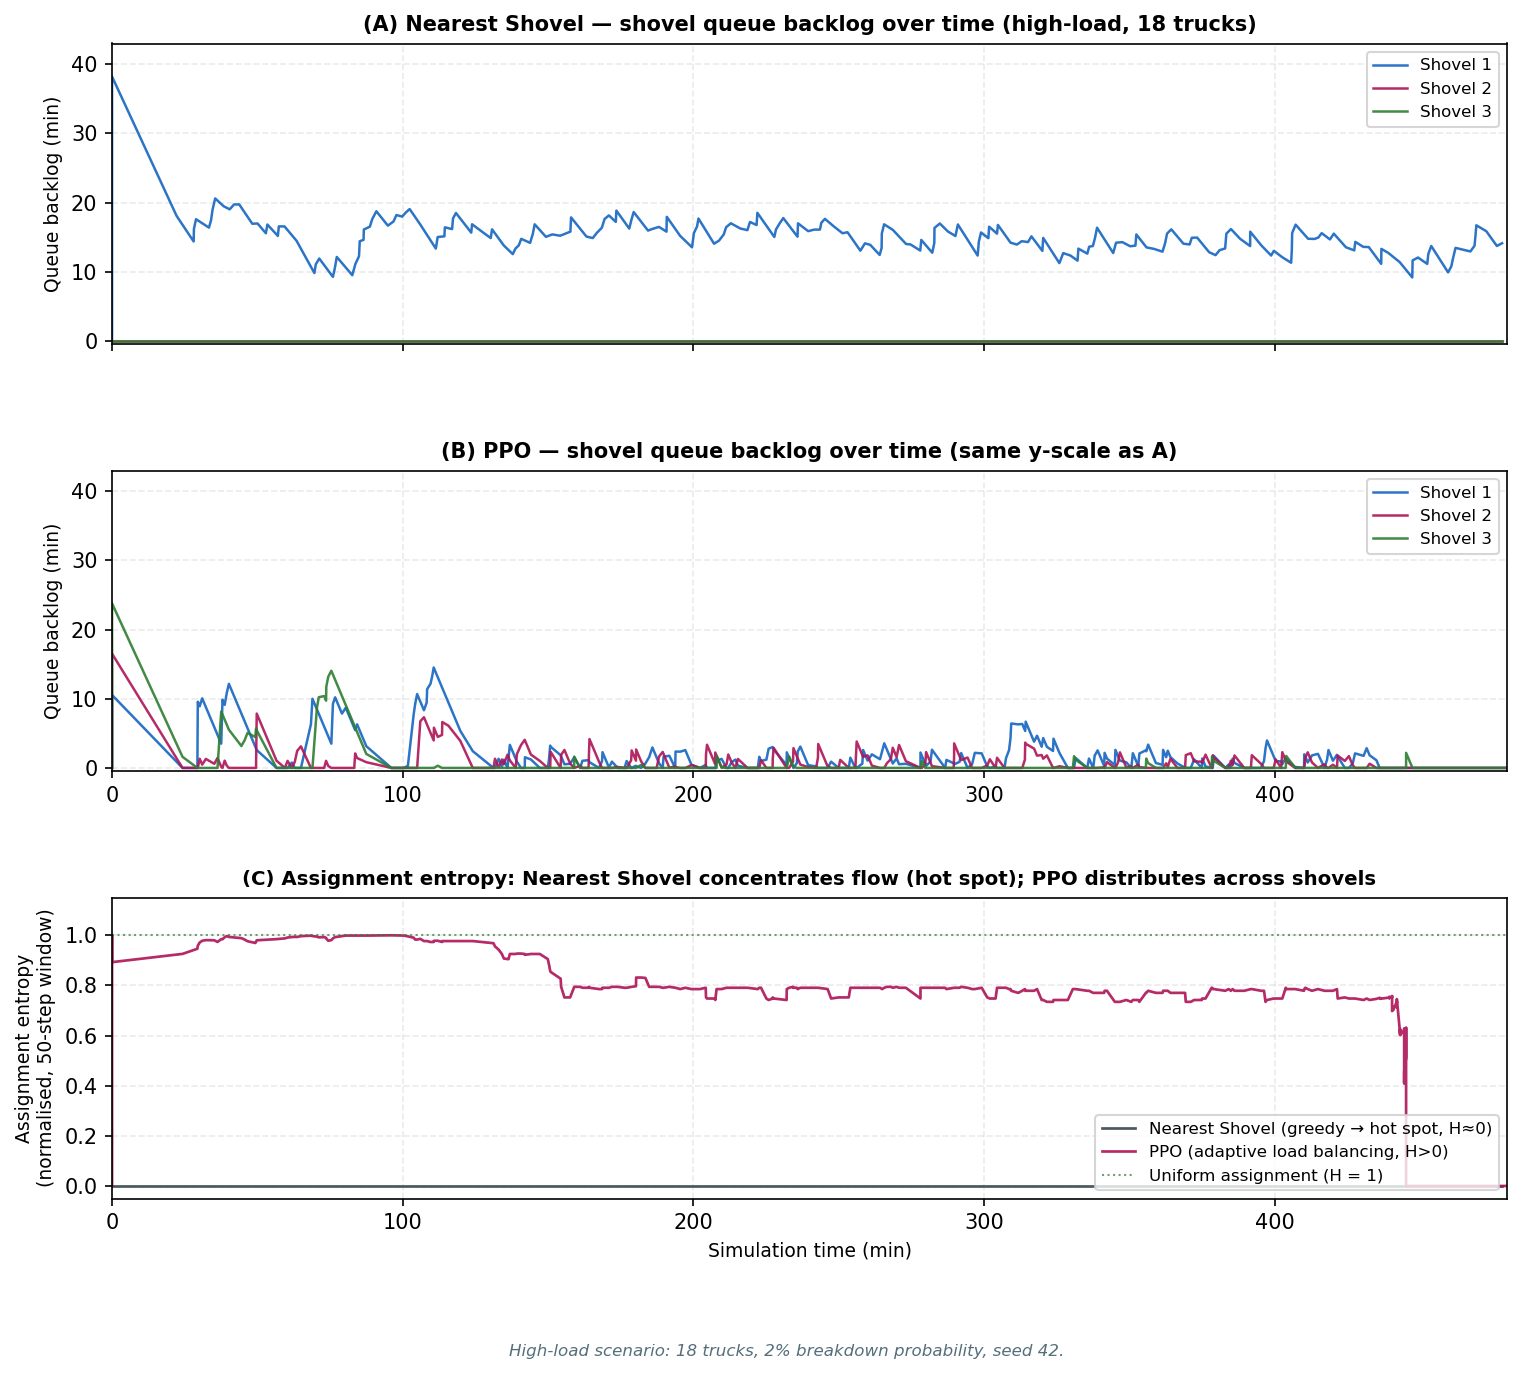
\includegraphics[width=0.96\textwidth]{figures/behavioral_analysis.png}
\caption{Behavioural analysis of Nearest Shovel and PPO under high load. Single episode with 18 trucks and seed 42. Panels (A) and (B) share the same $y$-axis scale; panel (C) reports the normalised assignment entropy, where $H=1$ corresponds to a uniform assignment across shovels.}
\label{fig:behavioral}
\end{figure}

\subsection{Industrial implications}

The integration of DRL into mining fleets should be viewed as a complementary decision layer rather than as a full replacement of existing FMS.

\begin{itemize}
  \item \textbf{Recommendation mode:} initially, DRL agents should operate in ``recommendation mode'', providing optimised assignment suggestions to human dispatchers or to autonomous haulage controllers. This enables a hybrid approach in which AI handles complexity while humans retain oversight.
  \item \textbf{Pre-deployment validation:} the significant performance gaps observed across scenarios underline the need for rigorous offline validation using digital twins before any real-world implementation.
  \item \textbf{Human intervention:} maintaining human control remains essential, particularly during the transition period, in order to manage edge cases that the simulation could not cover.
  \item \textbf{Application to large fleets and high-volume datasets:} applying the proposed approach at industrial scale (fleets of 50--200 trucks typical of mega open-pit operations) raises both computational and data-management challenges. On the computational side, the flat MLP architecture used here scales poorly with fleet size: the state dimension grows linearly with the number of trucks, and training time scales super-linearly with the number of interaction steps required for convergence at larger problem sizes. A Graph Neural Network (GNN) encoder that operates on the road-network graph addresses the first issue by sharing parameters across nodes, while distributing the computation via multi-agent architectures addresses the second. On the data side, large fleets generate high-frequency telemetry (GPS positions, payload weight, shovel queue depths at sub-minute resolution) whose volume can reach terabyte scale over a year of operation at a single mine site. DQN's experience replay buffer is particularly well-suited to exploit this data richness: offline pre-training on historical dispatch logs followed by online fine-tuning in simulation could substantially reduce the exploration burden and narrow the sim-to-real gap. This is consistent with the throughput advantage of DQN over PPO under high-breakdown conditions observed in this study and suggests that, if confirmed at scale, DQN may be the more industrially deployable candidate for large mine sites with abundant historical data, though this extrapolation remains speculative and should be validated empirically.
\end{itemize}

\subsection{Sustainability}
\label{sec:sustainability}

Although this study focuses primarily on productivity, its sustainability implications are significant.
\cref{tab:efficiency} consolidates equipment utilisation and specific fuel consumption across the nominal (N), high-load (HL) and high-breakdown (HB) scenarios. These figures provide the quantitative basis for the discussion below; the corresponding pairwise Welch $t$-test statistics and confidence intervals are reported alongside each comparison.

\begin{table}[H]
\centering
\caption{Equipment utilisation and specific fuel consumption across all policies and scenarios, reported as mean $\pm$ standard deviation over 30 replications.}
\label{tab:efficiency}
\footnotesize\setlength{\tabcolsep}{3pt}
\begin{tabular}{lcccccc}
\toprule
\multirow{2}{*}{\textbf{Policy}}
  & \multicolumn{3}{c}{\textbf{Utilisation (\%)}}
  & \multicolumn{3}{c}{\textbf{Specific fuel (L/t)}} \\
\cmidrule(lr){2-4}\cmidrule(lr){5-7}
  & \textbf{N} & \textbf{HL} & \textbf{HB}
  & \textbf{N}     & \textbf{HL}    & \textbf{HB} \\
\midrule
FIFO            & 96.2 & 93.7 & \textbf{91.7}  & $0.0534\pm0.0006$ & $0.0546\pm0.0004$ & $0.0555\pm0.0007$ \\
Fixed           & \textbf{96.4} & \textbf{93.9} & 90.8  & $0.0431\pm0.0003$ & $\mathbf{0.0444\pm0.0004}$ & $0.0453\pm0.0006$ \\
Nearest Shovel  & 87.3 & 62.3 & 83.6  & $0.0430\pm0.0004$ & $0.0582\pm0.0006$ & $0.0445\pm0.0005$ \\
Shortest Path   & 86.8 & 61.3 & 83.1  & $0.0432\pm0.0004$ & $0.0588\pm0.0005$ & $0.0447\pm0.0006$ \\
Q-Learning      & 90.9 & 88.7 & 84.9  & $0.0482\pm0.0012$ & $0.0537\pm0.0010$ & $0.0534\pm0.0014$ \\
SARSA           & 89.0 & 78.6 & 86.6  & $0.0555\pm0.0009$ & $0.0612\pm0.0008$ & $0.0571\pm0.0014$ \\
DQN             & 91.7 & 90.5 & 85.8  & $\mathbf{0.0408\pm0.0006}$ & $0.0445\pm0.0004$ & $\mathbf{0.0419\pm0.0006}$ \\
PPO             & 94.5 & 79.5 & 86.0  & $0.0415\pm0.0006$ & $0.0475\pm0.0023$ & $0.0427\pm0.0008$ \\
\bottomrule
\end{tabular}
\end{table}

\begin{itemize}
  \item \textbf{Idle-time reduction:} DQN maintains a mean waiting time of 47.8~min in high-load, comparable to FIFO (45.2~min) and Fixed Assignment (43.2~min); Nearest Shovel (199.6~min) and Shortest Path (204.3~min) collapse under fleet saturation. The utilisation collapse of Nearest Shovel and Shortest Path in high-load (62.3\% and 61.3\%, vs 93.9\% for Fixed; \cref{tab:efficiency}) quantifies the direct throughput cost of congestion: trucks spend over a third of the shift idle in queues instead of hauling.
  \item \textbf{Specific consumption and potential emissions:} DQN achieves the lowest specific fuel consumption in the nominal scenario ($0.0408$~L/t, 95\%~CI~$[0.0406,\,0.0409]$) and the high-breakdown scenario ($0.0419$~L/t, 95\%~CI~$[0.0418,\,0.0421]$). Holm-corrected Welch $t$-tests confirm large and statistically significant advantages over Fixed Assignment: nominal $\Delta=-5.5\%$ ($p=3.00\times10^{-46}$, $d=3.50$, 95\%~CI of difference~$[-0.0026,\,-0.0020]$~L/t); high-breakdown $\Delta=-7.3\%$ ($p=2.92\times10^{-58}$, $d=3.95$, 95\%~CI~$[-0.0036,\,-0.0031]$~L/t). PPO also outperforms Fixed in nominal ($\Delta=-3.9\%$, $p=3.60\times10^{-33}$, $d=2.41$) and high-breakdown ($\Delta=-5.6\%$, $p=1.18\times10^{-36}$, $d=2.49$). In high-load, DQN and Fixed Assignment are essentially tied ($0.0445$ vs $0.0444$~L/t; 95\%~CI~$[0.0444,\,0.0446]$ vs $[0.0443,\,0.0445]$; $p=0.875$, n.s.), while PPO consumes more ($0.0475$~L/t, $+7.0\%$, $p<0.001$, $d=2.15$), consistent with its high-variance routing under fleet saturation. SARSA shows the worst fuel efficiency across all scenarios, reflecting its longer waiting times and higher idle consumption. The magnitude of the main fuel difference ($|\Delta|=0.0023$~L/t, DQN vs Fixed in nominal) corresponds to roughly 53~L saved per 1,000 tonnes of ore moved, a non-trivial operational saving at mine-scale throughput. The exceptionally large effect sizes ($d>3$) reflect the low within-policy variability of fuel consumption (CV~$<5\%$) relative to the between-policy difference. Since diesel combustion is the primary source of direct CO$_2$, NO$_x$ and particulate emissions from surface mining fleets, a policy that reduces specific consumption per tonne would in principle produce a proportional reduction in tailpipe emissions. However, all figures reported here are simulation-derived; no direct emissions measurement was performed. Field validation on a real mine site is required before any definitive claim of environmental improvement can be made.
\end{itemize}

\subsection{Limitations}
\label{sec:limitations}

Despite the rigour of this study, several limitations must be acknowledged:

\begin{itemize}
  \item \textbf{Simulation gaps and absence of real-mine validation:} the study relies entirely on a simulated environment and has not been validated on a real mine site. Several factors cannot be fully replicated in discrete-event simulation: unpredictable weather and visibility changes, variable operator behaviour, unmapped road events and ad-hoc maintenance decisions. These may substantially affect the transferability of the reported performance gains to operational conditions.
  \item \textbf{Fleet homogeneity:} our model assumes a largely homogeneous fleet. In practice, mines operate trucks of varying ages and capacities, which adds a further layer of complexity to the dispatching logic.
  \item \textbf{Simplified breakdown model:} failures are generated by a stationary stochastic process and do not account for wear-related dependencies or maintenance scheduling.
  \item \textbf{Discrete action space:} the agent is restricted to a discrete set of shovels and dump sites. Future work should explore continuous or hierarchical action spaces in order to better model complex intersections and multi-pit operations.
  \item \textbf{Relatively static road network:} although travel times are stochastic and roads degrade over time, the topology of the network itself remains fixed during an episode.
  \item \textbf{Algorithm selection:} this study focused on PPO, DQN and tabular reinforcement learning. Several competitive algorithms were not included: Soft Actor-Critic (SAC) \cite{Haarnoja2018, SampsonNwachukwu2025}, Advantage Actor-Critic (A2C), Importance-Weighted Actor-Learner Architecture (IMPALA), and multi-agent reinforcement learning (MARL) \cite{Zhao2025} for decentralised truck coordination. Comparative benchmarks against these methods represent an important avenue for future work.
  \item \textbf{Training budget of the tabular baselines:} the tabular agents were trained for 30,000 episodes, a budget within which they do not reach a convergence plateau (\cref{fig:convergence}). Their reported performance is therefore a lower bound, and the gap between tabular and deep agents should be read as a gap under a fixed practical budget rather than as a gap between converged optima.
  \item \textbf{Replication budget:} although 30 independent replications per (policy, scenario) cell provide sufficient statistical power for the comparisons reported here, this remains a practical ceiling. Policies with high variance under disruption, notably PPO under high-load ($\pm$325~t/h, \cref{tab:productivity}), would benefit from a larger replication budget to further tighten confidence intervals.
  \item \textbf{Scalability to large fleets and datasets:} the experiments used a limited fleet (12--18 trucks, 3 shovels) whose state space can be compactly represented. Scaling to mega-mines operating 50--200 vehicles induces a combinatorial explosion that renders tabular methods (Q-Learning, SARSA) completely intractable and challenges even function-approximation approaches such as DQN and PPO. Three complementary strategies are identified for future work. (i)~\textit{Graph Neural Network (GNN) encoders}: replacing the flat MLP with a GNN that operates on the mine road graph naturally handles variable-fleet sizes and would in principle generalise to previously unseen mine topologies without retraining from scratch. (ii)~\textit{Multi-agent reinforcement learning (MARL)}: decentralising dispatching so that each truck acts as an independent agent with local observations reduces the joint action space from $\mathcal{O}(|\text{shovels}|^{N})$ to $\mathcal{O}(|\text{shovels}|)$ per truck, at the cost of non-stationarity during training \cite{Zhao2025}. (iii)~\textit{Transfer learning and curriculum}: a policy trained on a small reference fleet can be fine-tuned on a larger fleet using a fraction of the total training budget, provided the state encoding is fleet-size-agnostic. From a data perspective, larger fleets generate proportionally richer interaction logs (more transitions per episode), which benefits experience-replay methods such as DQN more than on-policy methods such as PPO, consistent with the robustness advantage observed here for DQN under high-breakdown conditions, whose causal attribution to the replay mechanism remains to be established by ablation.
\end{itemize}

% ============================================================================
% Section 8: Conclusion
% ============================================================================
\section{Conclusion and Future Work}
\label{sec:conclusion}

This study addressed the critical question of whether deep reinforcement learning policies can improve the productivity and operational resilience of truck--shovel systems compared with traditional industrial heuristics. By comparing eight distinct dispatching policies across three stochastic operational regimes (nominal, high-load and high-breakdown), we provided a comprehensive evaluation of adaptive logistics in open-pit mining.

The methodology relied on a Gymnasium-based custom stochastic open-pit mining simulator integrating stochastic travel times and equipment failure models, together with a statistical protocol based on 30 independent replications, common random seeds, Welch ANOVA (nominal scenario) and Kruskal--Wallis (disrupted scenarios), Dunn post-hoc tests with Holm--Bonferroni correction, and bootstrap confidence intervals. The main results reveal a nuanced picture. Under nominal conditions, the PPO agent achieved the highest productivity (4,176.67 t/h), a 2.6\% improvement over Fixed Assignment, while Fixed Assignment itself achieved the lowest mean waiting time (29.4 min), demonstrating that adaptive and rule-based policies are competitive on different metrics. Under fleet oversaturation, a \textit{congestion collapse} was observed exclusively for distance-based heuristics (Nearest Shovel: 199.6 min, Shortest Path: 204.3 min), while queue-based heuristics (FIFO, Fixed Assignment) and DRL agents maintained waiting times below 100 min. Finally, DQN achieved the highest absolute throughput in the high-breakdown regime (3,949.17 t/h, $\Delta=4.49\%$), leading PPO by 49.6~t/h ($d=0.636$, 95\,\% CI $[21.4,\,77.8]$~t/h; Welch $p=5.4\times10^{-4}$, though the primary rank-based Dunn post-hoc test yields $p=0.686$, well above the $\alpha=0.05$ threshold and therefore not significant). DQN's experience replay buffer may contribute to this advantage by allowing the agent to reuse transition states involving breakdown events across multiple gradient updates, a mechanism unavailable to the on-policy PPO agent. This remains a mechanistic hypothesis consistent with the data rather than a confirmed causal claim. SARSA exhibits the best relative robustness ratio ($\text{RR}_{\mathrm{HB}}=0.966$, $\Delta=3.38\%$), though this reflects its lower nominal baseline rather than genuine adaptive resilience. Among the top-performing policies, PPO degrades most ($\Delta=6.63\%$), ahead of Fixed Assignment ($\Delta=6.22\%$) and DQN ($\Delta=4.49\%$), while Q-Learning ($\Delta=11.30\%$) illustrates that tabular RL does not transfer well to disrupted dynamics.

The main scientific contribution of this research is to demonstrate that operational resilience constitutes a performance dimension in its own right, distinct from nominal efficiency. We showed that the optimal dispatching strategy is regime-dependent: a strategy that excels under stable conditions is not necessarily the most robust under disruption. This finding underlines the need for fleet management systems to move away from local, static optimisation rules towards adaptive, globally aware agents capable of anticipating delay propagation across the haulage network.

The principal limitation of this work is the absence of validation on a real mine site. All results are derived from a custom stochastic open-pit mining simulator; the sim-to-real gap persists, particularly with respect to unpredictable operator behaviour, ground-level variability and unmapped road events. Field deployment will require a rigorous calibration phase on operational data.

Consequently, near-term future work should focus on developing hierarchical or multi-agent reinforcement learning frameworks in which each truck operates as a decentralised agent equipped with local sensing and global coordination. The next validation step will consist in testing these policies on a digital twin calibrated with real operational data from an active mine site. Such a transition will be essential to verify the scalability of DRL agents to hundreds of vehicles and to quantify their direct impact on fuel consumption and carbon emissions in a physical mining environment. Ultimately, this research paves the way for the next generation of autonomous, resilient and sustainable mining logistics.

\newpage

% ============================================================================
% Sections finales
% ============================================================================
\section*{Data Availability}

The synthetic datasets generated during the present study, including simulation logs and performance indicators for the different operational scenarios, are available from the corresponding author upon reasonable request.

\section*{Code Availability}

The source code of the stochastic mining simulator, the training/evaluation scripts, the hyperparameter YAML files in the \texttt{configs/} directory, and the exact seed list used for the 30 replications (seeds 42--71) are publicly available on GitHub at \url{https://github.com/Juan-Lucas/memoire-master-rl-logistique}.

\section*{Author Contributions}

\textbf{Jean-Luc MUPASA KALUNGA:} conceptualisation, methodology, software, validation, formal analysis, investigation, writing (original draft), visualisation.

\textbf{Dr Olfa FERCHICHI:} supervision, conceptualisation, methodology, writing (review and editing), project administration.

\section*{Conflict of Interest}

The authors declare that they have no known competing financial interests or personal relationships that could have appeared to influence the work reported in this paper.

% Bibliographie
% \nocite{*}  % removed: all references are cited explicitly in the text
\bibliographystyle{plain}
\bibliography{RL_references}

% ============================================================================
% LISTE DES CLES DE CITATION UTILISEES (a verifier contre RL_references.bib)
% ---------------------------------------------------------
% Afrapoli2017            -> Afrapoli & Askari-Nasab, 2017 (FMS review)
% AlexandraNewman2010     -> Newman et al., 2010 (OR in mine planning)
% MohanMunirathinam1994   -> Munirathinam & Yingling, 1994
% Alarie2002              -> Alarie & Gamache, 2002
% Subtil2011              -> Subtil et al., 2011
% MehrnazMohtasham2023    -> Mohtasham & Mirzaei-Nasirabad, 2023
% NecmettinCetin2004      -> Cetin, 2004 (PhD thesis)
% MarceloFioroni2008      -> Fioroni et al., 2008
% Zeng2022                -> Zeng et al., 2022
% MiladAbolghasemian2020  -> Abolghasemian et al., 2020
% Soumis1989              -> Soumis et al., 1989
% Ahangaran2012           -> Ahangaran et al., 2012
% ChungTa2013             -> Ta et al., 2013
% AmandaSmith2020         -> Smith et al., 2020
% ZhongxinWang2022        -> Wang et al., 2022
% Souza2010               -> Souza et al., 2010
% GuangweiLiu2019         -> Liu & Chai, 2019
% BurakOzdemir2019        -> Ozdemir & Kumral, 2019
% ShivPrakashUpadhyay2017 -> Upadhyay & Askari-Nasab, 2017
% RichardSutton2018       -> Sutton & Barto, 2018
% MoezKrichen2022         -> Krichen, 2022
% MohammadrezaNazari2018  -> Nazari et al., 2018
% CongZhang2020           -> Zhang et al., 2020
% Hazrathosseini2024      -> Hazrathosseini & Afrapoli, 2024
% deCarvalho2023          -> de Carvalho & Dimitrakopoulos, 2023
% Banerjee2025            -> Banerjee et al., 2025 (Mining-Gym)
% Zhao2025                -> Zhao et al., 2025 (hierarchical MARL)
% Pei2025                 -> Pei et al., 2025
% FranciscoRosales2025    -> Rosales & Diaz, 2025
% JohnSchulman2017        -> Schulman et al., 2017 (PPO)
% MarkTowers2025          -> Towers et al., 2025 (Gymnasium)
% AntoninRaffin2021       -> Raffin et al., 2021 (Stable-Baselines3)
% SampsonNwachukwu2025    -> Nwachukwu et al., 2025 (SAC vs DDPG)
% KingaSzatmari2025        -> Szatmari et al., 2025 (cite en 2.3 et dans le tableau)
% ============================================================================

\end{document}